%\newcommand{\nl}{$n_{\hat{\ell}}$ }
\chapter{Émergence de la propriété petit-monde dans le modèle de Newman-Watts}
%\newcommand{\nl}{$n_{\hat{\ell}}$ } 
\label{sec3}
\begin{minipage}{\textwidth}
	\linespread{1.2}
	\minitoc
\end{minipage}
\section{Introduction}

Le modèle de Watts-Storogatz (WS) retient une attention particulière depuis son apparition en 1998 \cite{Watss-Strogatz1998}, il a deux propriétés très intéressantes: la présence d'un coefficient de Clustering élevé et d'un petit plus court chemin (propriété ou effet petit monde). Ces deux propriétés se trouvent dans la plupart des réseaux réels \cite{Cohen-Havlinl2010,Newman2010}, en plus ce modèle est très simple et combine la régularité avec l'aléatoire. En $1999$ Newman et Watts \cite{Newman-Watts1999} ont apporté une petite modification à ce modèle qui a faciliter l'analyse théorique pratiquement sans perdre aucune caractéristique.\\
L'émergence de la propriété petit-monde dans ces modèles est encore un phénomène pas bien compris, parmi ses problématiques on cite: à partir de quel point le réseau change sa nature grand-monde vers petit-monde ? si le réseau se sature par les raccourcis ajoutés ? comment et quand la saturation se réalise ? existe t-elle  une transition de phase ?. \\
Dans ce chapitre, nous aborderons quelques unes de ces questions. Dans nos calculs, nous utiliserons les techniques du groupe de renormalisation, et de la théorie de champ moyen. Les résultats analytiques sont  comparés aux simulations.

 \subsection{Modèle de Watts-Strogatz}
 
 
 Le modèle d'ER (voir section) reproduit l'effet petit monde (distance moyenne entre les nœuds est petite) observé dans les réseaux complexes, mais le coefficient de Clustering dans ce modèle est très faible par rapport à celui observé dans les systèmes réels, et la distribution des degrés est déférente des celle des réseaux réels. En 1998 Watts et Strogatz \cite{Watss-Strogatz1998} ont proposé un modèle qui reproduit deux propriétés parmi celles mentionnées précédemment de manière simple. Ce modèle, nommé souvent "petit-monde", peut être construit sur des réseaux de n'importe quelle dimension ou topologie, mais le cas le mieux étudié est l'unidimensionnel. Soit $n$ le nombre de nœuds et $k$ un nombre entier, le modèle Watts-Strogatz commence par la construction suivante (voir Fig.\ref{SW1}): 
 
 \begin{itemize}
 	\item Placez tous les nœuds en cercle;
 	\item Connectez chaque nœud à ses premiers $2k$ voisins les plus proches ($k$ voisins à droite, et $k$ voisins à gauche);
 	\item  Avec une probabilité $\phi$, chaque lien du réseau est enlevé, et ensuite placé entre deux nœuds choisis au hazard, ces nouveaux liens sont appelés raccourcis.
 \end{itemize}
 \begin{figure}[h!]
 	\centering
 	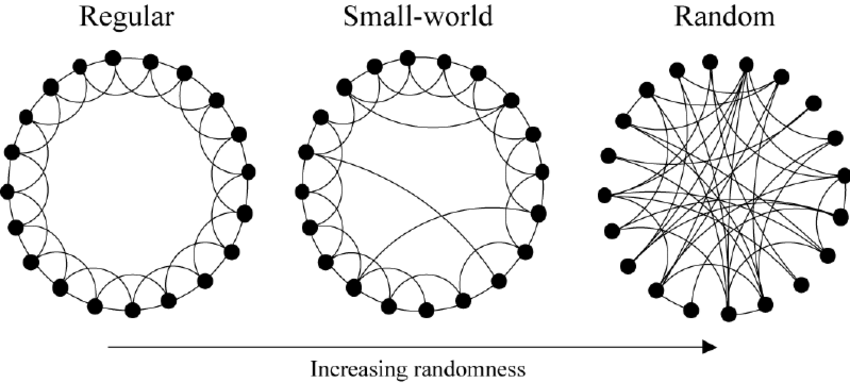
\includegraphics[scale=0.45]{./figures/fig-SW3}
 	\caption{Représentation schématique de l'évolution du processus de "reconnexion" dans le modèle Watts-Strogatz. Le nombre de nœuds est $n=20$ et $k=2$.}  	
 	\label{SW1}
 \end{figure}
 
 Ce modèle peut être justifié par le fait que la plupart des gens sont amis avec leurs voisins immédiats, par exemple les voisins de la même rue ou des collègues du même bureau. D'autre part, beaucoup de gens ont quelques amis qui habitent loin de leur quartier. Les propriétés structurelles du modèle sont quantifiées par le plus court chemin et le coefficient de clustering en fonction de la probabilité de reconnection.$\phi$.\\
 Le réseau régulier avec $\phi=0$ est un grand-monde, c'est-à-dire que la distance moyenne entre les nœuds se fait grande lorsque le nombre de nœuds $n$ devient grand, en effet, $\textless \ell \textgreater=\frac{2n}{k}$. Si $\phi=1$, le modèle de WS est équivalent au réseau aléatoire d'ER. Dans ce cas, le réseau est un petit-monde car $\textless {\ell} \textgreater \sim \ln(n)$.\\ 
 \begin{figure}[h!]
 	\centering
 	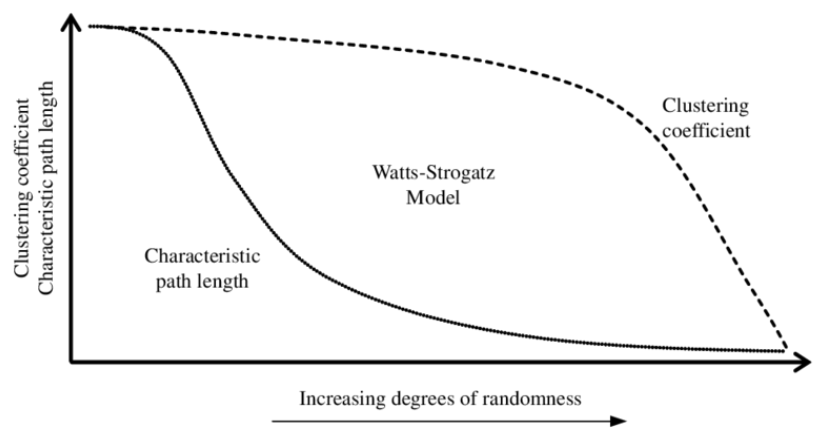
\includegraphics[scale=0.45]{./figures/fig-SW5}
 	\caption{Représentation de la variation de la longueur moyenne du chemin et du coefficient de regroupement avec la probabilité de reconnexion $\phi$ dans le modèle Watts-Strogatz.}  	
 	\label{SW2}
 \end{figure}
 La Fig.~\ref{SW2} \cite{Watss-Strogatz1998}, montre que la présence de
 quelques raccourcis entraîne la diminution de $\textless {\ell} \textgreater$. Le
 coefficient de clustering reste pratiquement inchangé pour les petites valeurs de 
 $\phi$, m\^{e}me si $\textless {\ell} \textgreater$ chute rapidement. L'implication importante est que la distance moyenne entre les nœuds chutte rapidement et devient petite pour les mêmes valeurs de $\phi$ auxquelles le Clustering local du réseau est significativement important. Ce modèle permet donc de construire des réseaux exhibant des propriétés observées dans les réseaux complexes naturels, petit plus court chemin  et grand coefficient de clustering, dépassant ainsi le modèle d’ER.\\
 Newman et Watts, en utilisant la transformation de groupe de renormalisation ont montré que le plus court chemin suit la loi universelle \cite{Newman-Watts1999-2}:
 \begin{equation}
 \textless\ell\textgreater= \frac{n}{k}f(x),
 \label{fc_univ}
 \end{equation}
 avec $x=nk\phi$ est le nombre moyen de raccourcis dans le réseau et $f(x)$ une fonction universelle.\\ 
 Le coefficient de clustering, C, est défini par l'Eq.~\eqref{Clustering}. 
 Pour évaluer $C$, nous devons calculer le nombre de triangles et de triplets connectés dans le réseau, Barrat a trouvé une très bonne approximation pour $C$ qui s'écrit sous la forme \cite{Barrat-Weigt2000}:
 \begin{equation}
 C=\frac{3(k-1)}{2(2k-1)}(1-\phi)^3.
 \end{equation}  
 Lorsque $\phi=0$, la distribution de degrés est une fonction delta centrée sur la valeur $2k$, alors que pour $\phi=1$ elle est similaire à celle d'un réseau ER. Pour les valeurs intermédiaires de $\phi$, la distribution de degrés est donnée par \cite{Barrat-Weigt2000}:
 \begin{equation}
 P(j)=\sum_{i=0}^{\text{min}(j-2k,m)}C_i^{2k}\frac{(2k\phi)^{j-2k-i}}{(j-2k-i)}e^{2k\phi}.
 \end{equation} 
 
%\section{La théorie de groupe de renormalisation et les transitions de phase}
%\end{sloppypar}
%Dans un système physique proche d'une transition de phase, les méthodes d'approximations les plus courantes s'appuyant à négliger les corrélations entre un grand nombre de particules ou plutôt entre un grand nombre des degrés de liberté, ces approximations sont valables lorsque la longueur de corrélation est petite. En pratique, on sait traiter de façon simple les corrélations entre deux particules. Le problème avec trois particules est déjà beaucoup plus difficile. Ce type de méthodes est voué à l'échec quand la longueur de corrélation est grande.

%D'où l'idée de réduction du nombre des degrés de liberté, on cherche à établir une correspondance entre un problème de longueur de corrélation donnée et un problème de longueur de corrélation plus petite. La théorie de groupe de renormalisation établit ainsi des correspondances entre systèmes de longueurs de corrélation différentes. Considérons par exemple un système de moments magnétiques en interaction au voisinage du point critique de la transition ferromagnétique. Afin de réduire le nombre élevé des degrés de liberté, au lieu de considérer tous les moments magnétiques atomiques individuellement, on les regroupe en blocs comprenant plusieurs moments que l'on considère comme nouvelles entités de base, avec un nouveau moment (moment de bloc). On calcule alors les interactions entre ces nouvelles entités, ce qui suppose qu'on a su moyenner les fluctuations des variables internes à l'intérieur des blocs. On change ensuite d'échelle de façon que le nouveau réseau devient le même que le précédent , enfin, on renormalise judicieusement la taille des nouveaux moments magnétiques. Une série d'opérations fait passer un système à un autre avec réduction de la longueur de corrélation. Dans cette transformation, les degrés de liberté du système sont diminués car on a moyenné les fluctuations des variations internes des blocs. Autrement dit on a remplacé l'interaction initiale entre les anciens degrés de liberté par une nouvelle interaction effective entre les degrés de liberté réduit \cite{Pelissetto-Vicari2002,Wilson1975}.\\
%Une définition formelle des transformations du groupe de renormalisation est un sujet complexe qui nécessite des développements mathématiques allant bien au delà du but de cette thèse, alors on se contente d'exposer l'idée générale de cette théorie importante qu'on utilisera dans nos calculs. 

%\section{Plus court chemin et transition de phase dans le modèle de WS(NW)}
\subsection{Modèle de Newman-Watts}
Newman et Watts (NW) \cite{Newman-Watts1999} ont introduit une petite modification au le modèle WS. Sans supprimer des liens, un raccourci connectant $2$ nœuds choisis au hazard est ajouté avec une probabilité $\phi$. En moyenne il y a $x=nk\phi$ raccourcis. Ce modèle a les m\^{e}mes propriétés que celui de WS, sauf pour $k=1$ où il y a une certaine différence (Expliquer, Quelles propriétés?)\footnote{Le cas $k=1$ est sans intérêt dans ce modèle car le coefficient de clustering est zéro}. En outre, le modèle de NW est plus abordable du point de vue du traitement analytique. En effet, par exemple, Newman a donné l'expression exacte du coeffcient de clustering \cite{Newman2010}:
\begin{equation}
C=\frac{3(k-1)}{4(k-1)+8k\phi+4k\phi^2}.
\end{equation}
	\begin{figure}[h!]
		\centering
		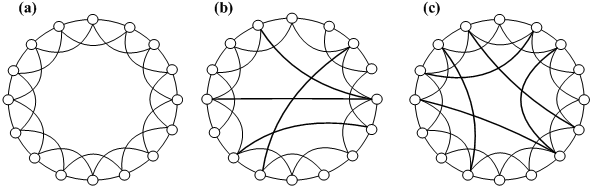
\includegraphics[scale=0.55]{./figures/fig-NW}
		\caption{Représentation schématique de l'évolution du processus de "reconnexion" dans le modèle NW.  Le nombre de nœuds est $n=20$ et $k=2$.}  	
		\label{NW}
	\end{figure}
En ce qui concerne le plus court chemin, il n'existe pas encore un calcul exacte dans le modèle de NW, et ça malgré sa simplicité apparente. Le traitement le plus important date de l'année $2000$ où Newman et al. \cite{Newman-al2000}, et avec un calcul de champ moyen très élaboré, ont trouvé une approximation de la fonction universelle Eq.~\eqref{fc_univ} sous la forme:
\begin{equation}
f(x)=\frac{1}{2\sqrt{x^2+2x}}\tanh^{-1}(\sqrt{\frac{x}{x+2}}),\label{eq-ws}
\end{equation}
les formes asymptotiques de cette fonction sont: 
\begin{align}
f(x)&\sim
\begin{cases}
\dfrac{1}{4} & \text{si } x \ll1\\
\\
\dfrac{\log\mathrm{2x}}{\mathrm{4x}}& \text{si } x \gg1.
\end{cases}
\end{align}
La fonction $f(x)$ s'avère exacte dans la limite de $n$ grand pour une densité de raccourcis donnée, ou dans la limite de la densité de raccourcis faible pour une taille $n$ donnée. Dans le cas où la densité des raccourcis est faible avec un nombre total de raccourcis grand (car le réseau lui-même est également grand), $f(x)$ est également une solution exacte. Au voisinage de $\phi=1$ une déviation entre cette solution  et les simulations numériques est observée (voir Fig.~\ref{chemin}). Dans la section suivante, nous proposons une explication inédite de l'origine de cette déviation.\\
Une des questions très étudiée dans le modèle de WS est l'existence de la transition de phase lors du passage du grand-monde pour $\phi=0$ au petit-monde pour $\phi=1$. 
En $1999$ Barthélémy et Amaral \cite{Barthelemy-Amaral1999} ont suggéré que la distance moyenne $\textless {\ell} \textgreater$ entre deux sommets quelconques du réseau est une fonction de $\frac{n}{n^*}$, où la taille de croisement(crossover) $n^*$ au-dessus de laquelle le réseau vérifie l'effet petit-monde ($\textless {\ell} \textgreater\sim \ln(n)$) se comporte pour $p\ll1$ comme $n^*\sim p^{-\tau}$ avec $\tau \approx \frac{2}{3}$. Ces auteurs ont affirmé qu'il s'agit plutôt d'un phénomène de crossover, et non d'une transition de phase. Barrat \cite{Barrat} argumente que $\tau$ ne peut pas être inférieur à $1$, il donne la  valeur $\tau=1$ en utilisant la m\^{e}me approche que Barthélémy et Amaral mais avec des tailles du système plus grandes. Newman et Watts \cite{Newman-Watts1999-2,Newman-Watts1999-3} confirment cette valeur de l'exposant critique  ($\tau=1$) en utilisant une transformation de groupe de renormalisation. Ces derniers suggèrent que la transition vers le petit-monde se fait d'une façon continue, c'est-à-dire une transition de phase de deuxième ordre où le point critique correspond à une densité de raccourcis tendant vers zéro ($\phi \rightarrow 0$). D'autres auteurs \cite{Argollo-al2000} ont trouvé un résultat différent des précédents, ceux-ci obtiennent une transition de phase de première ordre au point $\phi=0$, à cause d'une discontinuité d'un certain paramètre d'ordre en ce point. \\
On en déduit qu'il existe encore un débat à propos du type de la transition de phase dans ce modèle. Dans la section suivante nous allons traiter cette question en détail en nous nous baseront sur le fait que le réseau de NW est un mélange de régularité et d'aléas.
%\section{Couches et plus court chemin dans le modèle de NW}
%Notre travail ici se consacre, au début, à faire une étude sur les couches dans le modèle NW en utilisant la transformation de groupe de renormalisation en espace réel (GR), (voir Fig.~\ref{RG}). Une couche $n_d$ est le nombre de nœuds ayant la distance $d$ autour d'un nœud arbitraire. Sachant que ce modèle est un mélange entre la régularité et l'aléas,
%nous proposons de séparer les couches selon deux types, couches-régulières $n_d^r$ qui représentent le nombre des nœuds restant dans leurs distances régulières initiales $d$ sans aucune influence par les raccourcis ajoutés et les  couches-aléatoires $n_d^{al}$ qui représentent le nombre des nœuds changeant leurs distances régulières vers une nouvelle distance $d$
%plus proche du nœud arbitraire à cause des raccourcis (voir Fig.~\ref{r-al}). En manipulant les expressions de ces couches, on trouvera que la somme des couches aléatoires $S_{al}$ et la somme des couches régulières $S_{r}$, pouvant également s'écrire sous  forme d'une fonction universelle comme le plus court chemin, $S_{al}=nh(x)$ et $S_{r}=n(1-h(x))$ avec $h(x)=1-\sqrt{\frac{\pi}{4x}}erf(\sqrt{x})$. 
%Sachant que la fonction $h(x)$ représente la fraction des nœuds appartenant aux couches-aléatoires, on la considerera comme un paramètre d'ordre, car elle varie entre $0$ et $1$ selon le degré de l'ordre et désordre dans le réseau. Si on prend $h(x)$ comme un paramètre d'ordre, on peut en déduire l'absence d'une transition de phase dans ce modèle mais un phénomène de croisement commence depuis $x=0$.\\

%Pour calculer le plus court chemin, $\hat{\ell}$, 
%nous utilisons les résultats précédents et nous considérons également, comme le cas des couches, que le plus court chemin est la somme du plus court chemin du réseau-régulier $\hat{\ell}_{r}$ et le plus court chemin du réseau-aléatoire  $\hat{\ell}_{al}$, $\hat{\ell}=\hat{\ell}_{al}+\hat{\ell}_r$, en se
% basant dans le calcul de $\hat{\ell}_{al}$ sur la supposition que le plus court chemin est la position de la couche maximale (voir Chapitre.~\ref{sec3}) et pour calculer $\hat{\ell}_r$ on utilise une approximation qui sera décrite plus tard, et on va trouver une expression du plus court chemin  plus précise par rapport à l'expression de Newman et al. (voir Fig.~\ref{chemin}).
%En plus nous allons démontrer que la formule universelle en fonction du nombre de raccourcis est valable sauf pour $y\ll1$, avec $y=2k^2\phi$ est un nouveau paramètre que l'on va définir plus tard. Ce résultat est très important, car on montrera que la fonction  universelle $f(x)$ qui a été considérée dans la communauté scientifique comme étant toujours exacte, \hat{n}est pas vraiment correcte. Cependant on remarque qu'une autre formule universelle, $g(y)=\frac{ln(n)}{\hat{\ell}}$, apparaît lorsque  $y$ \hat{n}est pas très inférieur à $1$. Cette nouvelle formule montre que la propriété petit-monde émerge d'une façon universelle en fonction de $y$ et pas en fonction de $x$.\\
%Tous ces résultats obtenus vont être bien détaillé dans la suite.

\section{Structure du réseau de NW: couches de voisins et plus court chemin }

\subsection{Couches de voisins}
On se propose d'étudier en détail le nombre de voisins  $\hat{n}_{\hat{\ell}}$ se trouvant  à une distance $\hat{\ell}$ d'un nœud arbitraire en applicant la transformation du groupe de renormalisation en espace réel (GR) sur le réseau (voir Fig.~\ref{RG}). \'{E}tant donné que le modèle de NW est un mélange de régularité et d'aléas, les couches vont être séparées en deux catégories: 
\begin{itemize}
\item[-] Couches régulières $\hat{n}_{\hat{\ell}}^r$ où la distance $\hat{\ell}$ entre le nœud racine et ses voisins n'a pas été changée par l'introduction des raccourcis.
\item [-] Couches aléatoires $\hat{n}_{\hat{\ell}}^{al}$ où la distance $\hat{\ell}$ entre le nœud racine et ses voisins a été changée par l'introduction des raccourcis (voir Fig.~\ref{r-al}).
\end{itemize}
La transformation du GR remplace le réseau de $n$ nœuds avec chacun un degré $k$ par un autre réseau avec un nombre de nœuds {$\hat{n}$}$=\frac{n}{k}$ de degré $\hat{k}=1$
(voir Fig.~\ref{RG})\footnote{Le degré de liberté est réduit, car dans le nouveau réseau le paramètre  $\hat{k}$  est toujours égale à $1$, c'est exactement l'idée principale de la théorie du groupe de renormalisation.}. Chaque ensemble de $k$ nœuds voisins (\textsf{amas}) est considéré comme un seul nœud. Après l'ajout des raccorucis avec la probabilité $\phi$, la probabilité qu'un nœud (\textsf{amas}) dans le nouveau réseau ($\hat{k}=1$ et $\hat{n}=\frac{n}{k}$) soit lié aléatoirement à un autre nœud (\textsf{amas})est $\hat{\phi}=1-\big(1-\frac{2k\phi}{n}\big)^{k^2}$, pour $n\gg k\phi$ on peut écrire $\hat{\phi}\approx \frac{2k^3\phi}{n}$. On note $P_r(\hat{\ell})$ la probabilité que la distance $\hat{\ell}$ entre un nœud quelconque et le noeud racine ne soit pas modifiée après l'ajout des raccourcis, et soit $P_{al}(\hat{\ell})$ la probabilité que la distance entre un nœud quelconque et le noeud racine devienne égale à $\hat{\ell}$ après l'ajout des raccourcis. Dans l'exemple de la Fig.~\ref{r-al}, les nœuds sombres sont ceux qui deviennent plus proches du nœud racine $R$ grâce au raccourci.\\ 
\begin{figure}[h!]
\centering
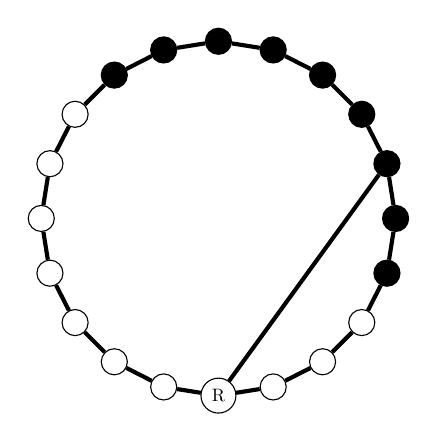
\begin{tikzpicture}[scale=0.25]
\tikzstyle{every node}=[scale=0.5,draw,shape=circle];
\node[scale=2,fill=black] (4) at (-18:9) {};
\node[scale=2,fill=black] (5) at (0:9) {};
\node[scale=2,fill=black] (6) at ( 18:9) {};
\node[scale=2,fill=black] (7) at (2*18:9) {};
\node[scale=2,fill=black] (8) at (3*18:9) {};
\node[scale=2,fill=black] (9) at (4*18:9) {};
\node[scale=2,fill=black] (10) at (5*18:9) {};
\node[scale=2,fill=black] (11) at (6*18:9) {};
\node[scale=2,fill=black] (12) at (7*18:9) {};
\node[scale=2] (13) at (8*18:9) {};
\node[scale=2] (14) at (9*18:9) {};
\node[scale=2] (15) at (10*18:9) {};
\node[scale=2] (16) at ( 11*18:9) {};
\node[scale=2] (17) at (12*18:9) {};
\node[scale=2] (18) at (13*18:9) {};
\node[scale=2] (19) at (14*18:9) {};
\node[scale=1.3] (r) at (15*18:9) {R};
\node[scale=2] (1) at (16*18:9) {};
\node[scale=2] (2) at (17*18:9) {};
\node[scale=2] (3) at (18*18:9) {};
\draw[line width=1.5pt](r)--(1)
(1) -- (2)
(2) -- (3)
(3) -- (4)
(4) -- (5)
(5) -- (6)
(6) -- (7)
(7) -- (8)
(8) -- (9)
(9) -- (10)
(10) -- (11)
(11) -- (12)
(12) -- (13)
(13) -- (14)
(14) -- (15)
(15) -- (16)
(16) -- (17)
(17) -- (18)
(18) -- (19)
(19) -- (r)
(r) -- (6);
\end{tikzpicture}
\caption{ Illustration des nœuds appartenant aux couches aléatoires (nœuds sombres) dont la distance au nœud racine $R$ a été changée par les raccourcis. Les nœuds appartenant aux couches réguliers (nœuds clairs) restent à la même distance de $R$ après introduction des raccourcis. Le réseau est de taille $n=20$, $k=1$, et avec un seul raccourci.}

\label{r-al}
\end{figure}

\noindent Généralement la réduction de la distance d'un nœud par rapport au nœud racine peut se faire à l'aide d'un seul, de deux ou plus de raccourcis. On note $\pi^m(i)$ la probabilité que la distance initiale d'un noeud ne soit pas changée  vers une distance plus petite $i$ à travers $m$ raccourcis. On distingue  les cas suivants:\\
\begin{itemize}
\item[$\blacksquare$]  Réduction de la distance par un raccourci:\\
Soit $\pi^1(i)$ la probabilité qu'un nœud $j$ ne change pas sa distance initiale $\hat{\ell}$ vers
la distance $i$ ($i<\hat{\ell}$) à travers un seul raccourci:
\begin{eqnarray}\nonumber
	\pi^1(1)&=&(1-\hat{\phi}), \\\nonumber
	\pi^1(2)&=&(1-\hat{\phi})^4,\\\nonumber
	\pi^1(3)&=&(1-\hat{\phi})^{4\cdot2},\\\nonumber
	\vdots\\
	\pi^1(i)&=&(1-\hat{\phi})^{4(i-1)},
	\label{pi1}
	\end{eqnarray}
dans $\pi^1(1)=(1-\hat{\phi})$ l'exposant est $1$ car il existe une seule possibilité pour que le nœud $j$ se lie directement au nœud racine $R$, pour $\pi^1(2)=(1-\hat{\phi})^4$  l'exposant est $4$ car pour que la distance entre $j$ et $R$ soit $2$, il faut que le nœud $j$ se lie directement à l'un des deux premiers voisins du nœud $R$ ou l'inverse, c'est-à-dire que $R$ se lie directement à l'un des premiers voisins de $j$, donc au totale $4$ possibilités. La déduction des autres probabilités se fait par le même raisonnement.
Le nombre de possiblités (sauts) pour construire un chemin tel que $\hat{\ell}=i$ est $4(i-1)$. Cette valeur est en général supérieure à la valeur réelle, car parmis ces possibilités il y en a qui correspondent à des distances $\hat{\ell}<i$ et qui sont déjà comptabilisées pour les distances inférieures. Lorsque le nombre de raccourcis est faible, le nombre de sauts ($4(i-1)$) est exacte. \\
De l'Eq.~\eqref{pi1} on déduit la probabilité $P^1_r(\hat{\ell})$ qu'un nœud ne change pas sa distance $\hat{\ell}$ à travers un seul raccourci:
\begin{eqnarray}\nonumber
P_r^1(\hat{\ell})&=&\pi^1(1)\pi^1(2)...\pi^1(\hat{\ell}-1)\\\nonumber
&=& (1-\hat{\phi})(1-\hat{\phi})^4(1-\hat{\phi})^{4\cdot2}...(1-\hat{\phi})^{4(\hat{\ell}-2)}\\\nonumber
&=&(1-\hat{\phi})^{1+4+4\cdot2+4\cdot3...4(\hat{\ell}-2)}\\
&=&(1-\hat{\phi})^{1+4\sum_{i=1}^{\hat{\ell}-1}(i-1)}.
\end{eqnarray}
Le terme  $\pi^i(i)=(1-\hat{\phi})^{i}(\hat{n}-2i)^{i-1}$, et par commodité de calcul, peut être négligé. Ceci  n'a pas d'influence sur le résultat car c'est une seule possibilité parmi beaucoup d'autres. Alors $P_r^1(\hat{\ell})$ s'écrit:
\begin{equation}
P_r^1(\hat{\ell})=(1-\hat{\phi})^{4\sum_{i=1}^{\hat{\ell}-1}(i-1)}.
\end{equation}
	
\item[$\blacksquare$]  \`{A} travers $2$ raccourcis: \\
Soit le noeud racine $R$ et un noeud $j$ quelconque, pour compter le nombre de possibilités pour aller de  $R$ à $j$ sachant qu'il y a deux raccourcis entre les deux noeuds, on introduit le noeud arbitraire $z$ qui se trouve entre les deux raccourcis. Dans ce cas, si la distance entre $R$ et $j$ en passant par $z$  est $i$, alors le nombre de possibilités est $i-1$, c'est-à-dire les cas $\{\{1,i-1\},\{2,i-2\},\cdots,\{i-1,1\}\}$. Pour $i=4$, par exemple, on a les trois cas suivants: $\{\{1,3\},\{2,2\},\{3,1\}\}$
\footnote{Les combinaisons possibles pour que la distance entre le nœud $j$ et le noeud racine $R$ soit $4$: \begin{itemize} \item[$\bullet$]la distance entre le nœud $R$ et le nœud intermédiaire $z$ est $1$ et entre $z$ et le nœud $j$ est $3$. \item[$\bullet$]la distance entre le nœud $R$ et le nœud intermédiaire $z$ est $2$ et entre $z$ et le nœud $j$ est également $2$. \item[$\bullet$]la distance entre le nœud $R$ et le nœud intermédiaire $z$ est $3$ et entre $z$ et le nœud $j$ est $1$.\end{itemize}}.
On peut schématiser le cas particulier $\{1,i-1\}$ comme:
\begin{figure}[h]
	\centering
	\begin{tikzpicture}[shorten >=1pt,auto,node distance=2cm,thick,main node/.style={circle,fill=black!20,draw}]
	%[-,>=stealth',shorten >=1pt,auto,node distance=2cm,thick,main node/.style={circle,fill=black!20,draw}]
	\node[main node] (1) {$z$};
	\node[main node,scale=0.85] (2) [left of=1] {$R$};
	\node[main node,scale=1.5] (3) [right of=1] {} ;
	\node[main node,scale=1.5] (4) [right of=3] {} ;
	\node[main node,scale=0.9] (5) [right of=4] {$j$} ;
	\draw[->,dashed] (4)--(5);
	\draw[->] (1)--(3);
	\draw[->] (3)--(4);
	\draw[->] (2)--(1) node[midway,below] {};
\draw [decorate,decoration={brace,mirror,amplitude=9pt},xshift=-4pt,yshift=0pt] (-1.8,-0.6) -- (0.24,-0.6) node [black,midway,yshift=-1cm,xshift=0cm] {\footnotesize $ \text{raccourci}$};
\draw [decorate,decoration={brace,raise=2pt,amplitude=9pt,mirror},xshift=0pt,yshift=0pt] (0.24,-0.5) -- (8,-0.5) node [black,midway,yshift=-1cm,xshift=0cm] {\footnotesize $i-1 \ \text{pas en présence d'un seul raccourci}$};

	\end{tikzpicture}
	
%	\caption{Estimation de .}
%	\label{}
\end{figure}
On constate que pour ce cas ($\{1,i-1\}$):
\begin{itemize}
	\item Le nombre de chemins possibles entre $R$ et $z$ est $1$ car ils sont directement liés à travers un raccourci.
	\item Le nombre de chemins possibles entre $z$ est $j$ est $4(i-2)$, car la distance entre eux est $i-1$ (voir le cas d'un seul raccourci).  
\end{itemize}
Dans ce cas, on déduit la probabilité pour que la distance entre les noeuds $R$ et $j$ ne soit pas égale à $i$ est $(1-\hat{\phi}^2)^{4(i-2)}$, où on a utilisé le fait que la probabilité pour que deux raccourcis se trouvent entre deux noeuds quelconques est $\hat{\phi}^2$.\\
Pour simplifier les calculs on suppose que tous les autres cas $\{\{2,i-2\},\cdots,\{i-1,1\}\}$ possèdent la mème probabilité que le cas $\{1,i-1\}$, ce qui représente une approximation de type champ moyen. Étant donné que le nombre de ces cas est $i-1$ alors la probabilité qu'un noeud ne change pas sa distance initiale vers la distance  $i$ via un certain noeud intermédiaire est $(1-\hat{\phi}^2)^{4(i-2)\times(i-1)}$.
Le nombre de positions possibles du noeud intermédiaire $z$ dans le réseau est $\hat{n}-2i$ (Fig.\ref{noeud-inter}), alors la probabilité qu'un noeud ne change pas sa distance initiale vers la distance  $i$ à travers deux raccourcis est 
\begin{eqnarray}
	\pi^2(i)=(1-\hat{\phi}^2)^{4(i-1)(i-2)(\hat{n}-2i)},
\end{eqnarray}
d'où
\begin{eqnarray}
	P_r^2(\hat{\ell})&=&\pi^2(1)\pi^2(2)...\pi^2(\hat{\ell}-1)\\\nonumber
	&=& (1-\hat{\phi}^2)^{4\sum_{i=1}^{i=\hat{\ell}-1}((i-1)(i-2)(\hat{n}-2i))},
\end{eqnarray}
le terme $\pi^2(2)$ est exclu de la somme comme expliqué dans le cas d'un seul raccourci.\\
	
	\begin{figure}[h!]
		\centering
		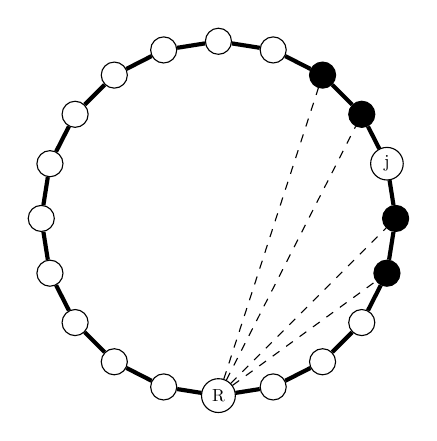
\begin{tikzpicture}[scale=0.25]
		\tikzstyle{every node}=[scale=0.5,draw,shape=circle];
		\node[scale=2,fill=black] (4) at (-18:9) {};
		\node[scale=2,fill=black] (5) at (0:9) {};
		\node[scale=1.3] (6) at ( 18:9) {j};
		\node[scale=2,fill=black] (7) at (2*18:9) {};
		\node[scale=2,fill=black] (8) at (3*18:9) {};
		\node[scale=2] (9) at (4*18:9) {};
		\node[scale=2] (10) at (5*18:9) {};
		\node[scale=2] (11) at (6*18:9) {};
		\node[scale=2] (12) at (7*18:9) {};
		\node[scale=2] (13) at (8*18:9) {};
		\node[scale=2] (14) at (9*18:9) {};
		\node[scale=2] (15) at (10*18:9) {};
		\node[scale=2] (16) at ( 11*18:9) {};
		\node[scale=2] (17) at (12*18:9) {};
		\node[scale=2] (18) at (13*18:9) {};
		\node[scale=2] (19) at (14*18:9) {};
		\node[scale=1.26] (r) at (15*18:9) {R};
		\node[scale=2] (1) at (16*18:9) {};
		\node[scale=2] (2) at (17*18:9) {};
		\node[scale=2] (3) at (18*18:9) {};
		\draw[line width=1.5pt](r)--(1)
		(1) -- (2)
		(2) -- (3)
		(3) -- (4)
		(4) -- (5)
		(5) -- (6)
		(6) -- (7)
		(7) -- (8)
		(8) -- (9)
		(9) -- (10)
		(10) -- (11)
		(11) -- (12)
		(12) -- (13)
		(13) -- (14)
		(14) -- (15)
		(15) -- (16)
		(16) -- (17)
		(17) -- (18)
		(18) -- (19)
		(19) -- (r);
		\draw[-,dashed] (r) -- (7);
		\draw[-,dashed] (r) -- (8);
		\draw[-,dashed] (r) -- (4);
		\draw[-,dashed] (r) -- (5);
		\end{tikzpicture}
		\caption{Représentation du cas $\{1,i-1\}$. Les nœuds sombres et les nœuds $j$ et $R$ sont les positions qui ne peuvent pas être occupés par le nœud intermédiaire. Étant donné que $\hat{n}=20$ et $i=3$,  le nombre de positions possibles pour le nœud intermédiaire est $\hat{n}-2i=14$.}
		
		\label{noeud-inter}
	\end{figure}
\item[$\blacksquare$]  \`{A} travers $3$ raccourcis:\\
Soit le nœud racine $R$ et un nœud $j$ quelconque, pour compter le nombre de possibilités pour aller de  $R$ à $j$ sachant qu'il y a trois raccourcis entre les deux noeuds, on introduit les noeuds arbitraires $z_1$ et $z_2$ qui séparent les trois raccourcis (voir figure) . Dans ce cas, si la distance entre $R$ et $j$ en passant par $z_1$ et $z_2$ est $i$, alors le nombre de possibilités est $C_2^{i-1}=\frac{(i-1)(i-2)}{2!}$, c'est-à-dire les cas $\{\{1,1,i-2\},\{1,2,i-3\},\cdots,\{i-2,1,1\}\}$. Pour $i=4$, par exemple, on a les trois cas suivants:$\{\{1,1,2\},\{1,2,1\},\{2,1,1\}\}$.
On peut schématiser le cas particulier $\{1,1,i-2\}$ par

\begin{figure}[h]
	\centering
	\begin{tikzpicture}[shorten >=1pt,auto,node distance=2cm,thick,main node/.style={circle,fill=black!20,draw}]
	\node[main node] (1) {$z_1$};
	\node[main node,scale=0.8] (2) [left of=1] {$R$};
    \node[main node,scale=0.9] (3) [right of=1] {$z_2$} ;
	\node[main node,scale=1.5] (4) [right of=3] {} ;
	\node[main node,scale=1.5] (5) [right of=4] {} ;
	\node[main node,scale=0.85] (6) [right of=5] {$j$} ;
	\draw[->,dashed] (5)--(6);
	\draw[->] (4)--(5);
	\draw[->] (1)--(3);
	\draw[->] (3)--(4);
	\draw[->] (2)--(1) node[midway,below] {};
	\draw[decorate,decoration={brace,mirror,amplitude=9pt},xshift=-4pt,yshift=0pt] (-1.8,-0.6) -- (0.24,-0.6) node [black,midway,yshift=-1cm,xshift=0cm] {\footnotesize $ \text{ raccourci}$};
	\draw[decorate,decoration={brace,raise=2pt,amplitude=9pt,mirror},xshift=0pt,yshift=0pt] (0.24,-0.55) -- (2,-0.55) node [black,midway,yshift=-1cm,xshift=0cm] {\footnotesize $\text{ raccourci}$};
	\draw[decorate,decoration={brace,raise=2pt,amplitude=9pt,mirror},xshift=0pt,yshift=0pt] (2.24,-0.55) -- (10,-0.55) node [black,midway,yshift=-1cm,xshift=0cm] {\footnotesize $i-2 \ \text{pas en présence d'un seul raccourci}$};
	
	\end{tikzpicture}
	
	%	\caption{Estimation de .}
	%	\label{}
\end{figure}

Pour le cas de la figure ($\{1,1,i-2\}$), on a:
\begin{itemize}
	\item Le nombre de chemins possibles entre $R$ et $z_1$ est $1$, car la distance entre eux est $1$.
	\item Le nombre de chemins possibles entre $z_1$ et $z_2$ est $1$, car la distance entre eux est $1$.
	\item Le nombre de chemins possibles entre $z_2$ et $j$ est $4(i-3)$, car la distance entre eux est $i-2$ (voir le cas d'un seul raccourci).  
\end{itemize}
On déduit que la probabilité du cas $\{1,1,i-2\}$ est $(1-\hat{\phi}^3)^{4(i-3)}$.
Comme dans le cas de deux raccourcis, pour simplifier les calculs on suppose que tous autres cas $\{\{1,2,i-3\},\cdots,\{i-2,1,1\}\}$ possèdent la mème probabilité que le cas $\{1,1,i-2\}$. Étant donné que le nombre de ces cas est $C_2^{i-1}=\frac{(i-1)(i-2)}{2!}$ alors la probabilité qu'un noeud ne change pas sa distance initiale vers la distance  $i$ via deux noeud intermédiaires quelconques est $(1-\hat{\phi}^3)^{4(i-2)\times\frac{(i-1)(i-2)}{2!}}$.
Le nombre de positions possibles des noeuds intermédiaires $z_1$ et $z_2$ dans le réseau est borné supérieurement par  $(\hat{n}-2i)^2$, alors la probabilité qu'un noeud ne change pas sa distance initiale vers la distance  $i$ à travers trois raccourcis est
	\begin{equation}
	\pi^3(i)=(1-\hat{\phi}^3)^{4\frac{(i-1)(i-2)}{2!}(i-3)(\hat{n}-2i)^2}
	\end{equation}
	  d'où
	\begin{eqnarray}
	P_r^3(\hat{\ell})&=&\pi^3(1)\pi^3(2)...\pi^3(\hat{\ell}-1)\\\nonumber
	&=& (1-\hat{\phi}^3)^{4\sum_{i=1}^{i=\hat{\ell}-1}(\frac{(i-1)(i-2)}{2!}(i-3)(\hat{n}-2i)^2)}.
	\end{eqnarray}
	
%\item[$\blacksquare$] \`{A} travers $4$ raccourcis:\\
%Dans ce cas on a trois nœuds intermédiaires $z$,$z'$ et $z''$, toujours sous la condition  qu'il y a un seul raccourci entre chaque deux nœuds
%intérimaires. La probabilité qu'un nœud ne change pas sa distance $j$ vers la $i^{\text{ème}}$ distance à travers $4$ raccourcis dans 
%le cas où le nœud arbitraire est lié directement par un raccourci avec $z$ et celui-ci est aussi directement lié par un raccourci 
%avec $z'$ qui est de sa part lié directement par un raccourci avec le nœud $z''$  et ce dernier à une distance de $i-3$ au
%nœud $j$ à travers aussi un seul raccourci est $(1-\hat{\phi}^4)^{4(i-4)}$.
%On considère comme les cas précédent que cette probabilité est la m\^{e}me
%pour les autres possibilités d'arrangements de quatre raccourcis autour les trois nœuds intermédiaires.\\ Le nombre d'arrangements possibles de ces quatre raccourcis
%autour les nœuds intérimaires $z$,$z'$ et $z''$ pour que la distance entre $j$ et le nœud  arbitraire est $i$ est
%$C_3^{i-1}=\frac{(i-1)(i-2)(i-3)}{3!}$.\\ En outre le nombre maximal  des positions possibles de $z$,$z'$ et $z''$ sur le réseau pour $i<j$ est  approximativement
%$(\hat{n}-2i)^3$.
%Alors on obtient
%\begin{eqnarray}
%	\pi^4(i)=(1-\hat{\phi}^4)^{4\frac{(i-1)(i-2)(i-3)}{3!}(i-4)(\hat{n}-2i)^3},
%	\end{eqnarray}
%	d'où
%	\begin{eqnarray}
%	%P_r^4(j)&=&\pi^4(1)\pi^4(2)...\pi^4(j-1)\\\nonumber
%	&=& (1-\hat{\phi}^4)^{4\sum_{i=1}^{i=j-1}(\frac{(i-1)(i-2)(i-3)}{3!}(i-4)(\hat{n}-2i)^3)}.
%	\end{eqnarray}
	
\item[$\blacksquare$] \`{A} travers $m$ raccourcis:\\
En suivant la même démarche que les cas précédents, on généralise facilement pour le cas de $m$ raccourcis. Dans ce cas on introduit $m-1$ noeuds intermédiaires, et on obtient: 
\begin{eqnarray}
	\pi^m(i)=(1-\hat{\phi}^m)^{4\frac{(i-1)(i-2)\ldots(i-m)}{(m-1)!}(\hat{n}-2i)^{(m-1)}},
\end{eqnarray}
alors la probabilité qu'un nœud ne change pas sa distance régulière $j$ à travers $m$ raccourcis est:
\begin{eqnarray}
	P_r^m(\hat{\ell})&=&\pi^m(1)\pi^m(2)...\pi^m(\hat{\ell}-1)\\\nonumber
	&=& (1-\hat{\phi}^m)^{4\sum_{i=1}^{\hat{\ell}-1}(\frac{(i-1)(i-2)\ldots(i-m)}{(m-1)!}(\hat{n}-2i)^{m-1})},
	\end{eqnarray}
puisque $\hat{\phi}<1$ on peut écrire 
\begin{eqnarray}
P_r^m(\hat{\ell})=e^{-4q^m\sum_{i=1}^{\hat{\ell}-1}(\frac{(i-1)(i-2)\ldots(i-m)}{(m-1)!}(\hat{n}-2i)^{m-1})}.
\end{eqnarray}
\end{itemize}
Alors la probabilité $P_r(\hat{\ell})$ qu'un nœud ne change pas sa distance régulière $\hat{\ell}$ après l'ajout d'un nombre quelconque de raccourcis est
\begin{eqnarray}
P_r(\hat{\ell})&=&P^1_r(\hat{\ell})P^2_r(\hat{\ell})P^4_r(\hat{\ell})\ldots P^{\hat{\ell}-1}_r(\hat{\ell})\\\nonumber
&=&e^{-4q\sum_{i=1}^{\hat{\ell}-1}(i-1)B(i)}, 
\end{eqnarray}
avec
\begin{eqnarray}
B(i)&=&1+[\hat{\phi}(i-2)(\hat{n}-2i)]+[\hat{\phi}^2\frac{(i-2)(i-3)}{2!}(\hat{n}-2i)^{2}]+\ldots+[\hat{\phi}^{i-2}(\hat{n}-2i)^{i-2}]\nonumber \\ \nonumber
	&=&1+[\hat{\phi}(i-2)(\hat{n}-2i)]+[\hat{\phi}^2\frac{(i-2)(i-3)}{2!}(\hat{n}-2i)^{2}]+\ldots+[\hat{\phi}^{i-2}(\hat{n}-2i)^{i-2}]\\ \nonumber
&=&\sum_{j=1}^{i-2}C_j^{i-2}[\hat{\phi}(\hat{n}-2i)]^j1^{i-2-j}\\ \nonumber 
&=&(\hat{\phi}(\hat{n}-2i)+1)^{i-2}.
\end{eqnarray}
qui n'est autre que la formule du binôme.
\begin{figure}[h!]
	\centering 
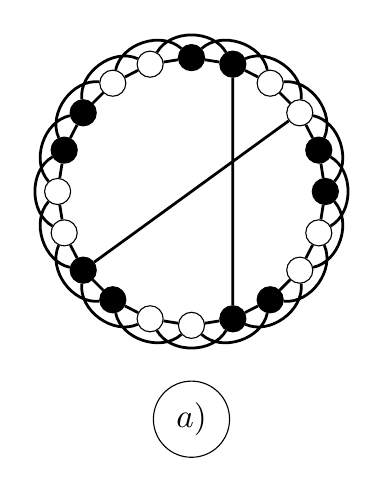
\begin{tikzpicture}[scale=0.2]
\draw (0,-12) node[scale=2,below]{$a)$} ;
\tikzstyle{every node}=[scale=0.5,draw,shape=circle];
\node[scale=2]  (4) at (-18:8.5) {};
\node[scale=2,fill=black] (5) at (0:8.5) {};
\node[scale=2,fill=black] (6) at ( 18:8.5) {};
\node[scale=2] (7) at (2*18:8.5) {};
\node[scale=2] (8) at (3*18:8.5) {};
\node[scale=2,fill=black] (9) at (4*18:8.5) {};
\node[scale=2,fill=black] (10) at (5*18:8.5) {};
\node[scale=2] (11) at (6*18:8.5) {};
\node[scale=2] (12) at (7*18:8.5) {};
\node[scale=2,fill=black] (13) at (8*18:8.5) {};
\node[scale=2,fill=black] (14) at (9*18:8.5) {};
\node[scale=2] (15) at (10*18:8.5) {};
\node[scale=2] (16) at ( 11*18:8.5) {};
\node[scale=2,fill=black] (17) at (12*18:8.5) {};
\node[scale=2,fill=black] (18) at (13*18:8.5) {};
\node[scale=2] (19) at (14*18:8.5) {};
\node[scale=2] (r) at (15*18:8.5) {};
\node[scale=2,fill=black] (1) at (16*18:8.5) {};
\node[scale=2,fill=black] (2) at (17*18:8.5) {};
\node[scale=2] (3) at (18*18:8.5) {};
\draw[line width=1pt](r)--(1)
(1) -- (2)
(2) -- (3)
(3) -- (4)
(4) -- (5)
(5) -- (6)
(6) -- (7)
(7) -- (8)
(8) -- (9)
(9) -- (10)
(10) -- (11)
(11) -- (12)
(12) -- (13)
(13) -- (14)
(14) -- (15)
(15) -- (16)
(16) -- (17)
(17) -- (18)
(18) -- (19)
(19) -- (r);
\draw[line width=1pt] (r) to [bend right=60] (2) 
(2)to [bend right=60](4)
(4)to [bend right=60](6)
(6)to [bend right=60](8)
(8)to [bend right=60](10)
(10)to [bend right=60](12)
(12)to [bend right=60](14)
(14)to [bend right=60](16)
(16)to [bend right=60](18)
(18)to [bend right=60](r)
(1)to (9)
(17)to (7)

(1)to [bend right=60](3)
(3)to [bend right=60](5)
(5)to [bend right=60](7)
(7)to [bend right=60](9)
(9)to [bend right=60](11)
(11)to [bend right=60](13)
(13)to [bend right=60](15)
(15)to [bend right=60](17)
(17)to [bend right=60](19)
(19)to [bend right=60](1);
\end{tikzpicture}
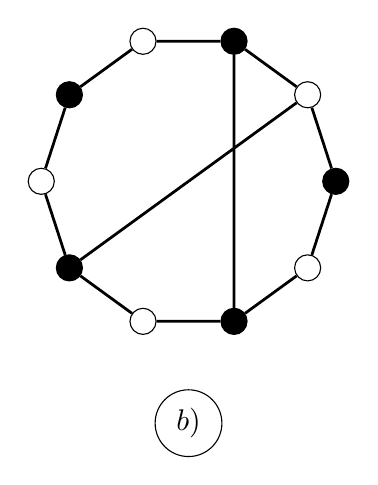
\begin{tikzpicture}[scale=0.22]
\draw (0,-12) node[scale=1.8,below]{$b)$} ;
\tikzstyle{every node}=[scale=0.5,draw,shape=circle];
\node (4)[scale=2] at (-36:8.5) {};
\node (5)[scale=2,fill=black]  at (0:8.5) {};
\node (6)[scale=2] at ( 36:8.5) {};
\node (7)[scale=2,fill=black]  at (2*36:8.5) {};
\node (8)[scale=2] at (3*36:8.5) {};
\node (9)[scale=2,fill=black]  at (4*36:8.5) {};
\node (r)[scale=2] at (15*36:8.5) {};
\node[scale=2,fill=black] (1) at (16*36:8.5) {};
\node (2)[scale=2] at (17*36:8.5) {};
\node[scale=2,fill=black]  (3) at (18*36:8.5) {};
\draw[line width=1pt](r)--(1)
(1) -- (2)
(2) -- (3)
(3) -- (4)
(4) -- (5)
(5) -- (6)
(6) -- (7)
(7) -- (8)
(3) -- (7)
(1) -- (6)
(8) -- (9)
(9) -- (r);
%\node[scale=3,text centered] at (0,-12) {b)};
\end{tikzpicture}
\caption{La transformation du GR d'un réseau (a) de $n=20$ et $k=2$ vers un réseau (b) de $\hat{n}=10$ et $\hat{k}=1$.}
\label{RG}
\end{figure}

Alors la probabilité qu'un nœud ne change pas sa distance $\hat{\ell}$ est: 
\begin{eqnarray}
\label{pr}
P_r(\hat{\ell})&=& e^{-4q\sum_{i=1}^{\hat{\ell}-1}(i-1)(\hat{\phi}(\hat{n}-2i)+1)^{i-2}}\\\nonumber
&\approx&e^{-4\hat{\phi}\int_{i=1}^{\hat{\ell}-1}(i-1)(\hat{\phi}(\hat{n}-2i)+1)^{i-2}di}.
\end{eqnarray}

La probabilité $P_{al}(\hat{\ell})$ qu'un nœud soit à une  distance $\hat{\ell}$ du nœud racine après l'ajout des raccourcis est égale au produit de la probabilité que ce nœud ne change pas sa distance vers une autre inférieure à  $\hat{\ell}$, $P_r(\hat{\ell}-1)$, par la probabilité que le nœud change sa distance vers la  distance $\hat{\ell}$, $1-\pi(\hat{\ell})$, avec $\pi(\hat{\ell})=\Pi^{\hat{\ell}-1}_{i=1}(\pi^i(\hat{\ell}))$.

\begin{eqnarray}\nonumber
P_{al}(\hat{\ell})&=&P_r(\hat{\ell}-1)(1-\pi(\hat{\ell}))\\\nonumber
&=&P_r(\hat{\ell}-1)-\pi(j)P_r(\hat{\ell}-1)\\\nonumber
&=&P_r(\hat{\ell}-1)-P_r(\hat{\ell})\\\nonumber
&=&-\frac{\partial P_r(\hat{\ell})}{\partial \hat{\ell}}\\
&=&4q(\hat{\ell}-2)(\hat{\phi}(\hat{n}-2(\hat{\ell}-1)-1))+1)^{\hat{\ell}-3}P_r(\hat{\ell}),
\end{eqnarray}
pour simplifier les calculs on peut prendre $\hat{\ell}-1\approx \hat{\ell}$ \footnote{Cette approximation représente une erreur de l'ordre de $\frac{1}{\hat{\ell}}$, or $\hat{\ell}$ tend vers l'infini lorsque $n$ est très large}, on obtient
\begin{eqnarray}
P_{al}(\hat{\ell})=4q(\hat{\ell}-1)(\hat{\phi}(\hat{n}-2\hat{\ell}-1))+1)^{\hat{\ell}-2}P_r(\hat{\ell}).
\label{pal}
\end{eqnarray}
Le nombre  moyen de nœuds dans la couche régulière $n_{\hat{\ell}}^r$ est $P_r(\hat{\ell})$ multiplié par $2$, car initialement dans chaque couche on a  deux nœuds réguliers à une distance $\hat{\ell}$
\begin{eqnarray}
n_{\hat{\ell}}^r=2P_r(\hat{\ell}),
\label{cr}
\end{eqnarray}
et le nombre de nœuds dans la couche aléatoire $n_{\hat{\ell}}^{al}$ est $P_{al}(\hat{\ell})$ multiplié par le nombre de nœuds qui sont à une distance plus grande que $\hat{\ell}$
\begin{eqnarray}
n_{\hat{\ell}}^{al}=(\hat{n}-2\hat{\ell})P_{al}(\hat{\ell}),
\label{cal}
\end{eqnarray}
d'où la $\hat{\ell}^{\text{ème}}$ couche qui est la somme des deux contributions s'écrit:

\begin{eqnarray}\nonumber
n_{\hat{\ell}}&=&n_{\hat{\ell}}^{r}+n_{\hat{\ell}}^{al}\\\nonumber
&=&2P_r(\hat{\ell})+(\hat{n}-2\hat{\ell})P_{al}(\hat{\ell})\\\nonumber
&=&2P_r(\hat{\ell})+(\hat{n}-2\hat{\ell})P_r(\hat{\ell}-1)-(\hat{n}-2\hat{\ell})P_r(\hat{\ell})\\\nonumber
&=&(\hat{n}-2\hat{\ell})P_r(\hat{\ell}-1)-(\hat{n}-2(\hat{\ell}+1))P_r(\hat{\ell})\\
&=&v(\hat{\ell}-1)-v(\hat{\ell}) \quad \quad  \text{avec:} \quad v(\hat{\ell})=(\hat{n}-2(\hat{\ell}+1))P_r(\hat{\ell}).
\label{c}
\end{eqnarray}
Pour quantifier la contribution des nœuds appartenant aux différentes couches (régulières et aléatoires) on calcule leurs sommes $\hat{S}_r$  et $\hat{S}_{al}$, ce qui permettra aussi de comparer les deux contributions:
\begin{eqnarray}\nonumber
\hat{S}_r &=&\hat{n}_{1}^{r}+\sum^{\frac{\hat{n}}{2}}_{\hat{\ell}=2}\hat{n}_{\hat{\ell}}^{r}\\\nonumber
&=&\hat{n}_{1}^{r}+\int^{\frac{\hat{n}}{2}}_2\hat{n}_{\hat{\hat{\ell}}}^{r}d\hat{\ell}\\
&=&\hat{n}_{1}^{r}+2\int^{\frac{\hat{n}}{2}}_2e^{-4q\int_{j=1}^{\hat{\ell}-1}(j-1)(\hat{\phi}(\hat{n}-2j)+1)^{j-2}dj}d\hat{\ell},
\label{ssr}
\end{eqnarray}
l'intégrale $\int^{\frac{\hat{n}}{2}}_2e^{-4q\int_{j=1}^{\hat{\ell}-1}(j-1)(\hat{\phi}(\hat{n}-2j)+1)^{j-2}dj}d\hat{\ell}$ n'a aucune solution explicite. Or lorsque le nombre de raccourcis $\hat{\phi}$ est grand $\hat{S}_r$ $\longrightarrow 0$ car presque tous les noeuds sont affectés par les raccourcis, on peut donc approximer l'intégrale précédente par le cas où $\hat{\phi}$ est faible, on a
$\int^{\frac{\hat{n}}{2}}_2e^{-4q\int_{j=1}^{\hat{\ell}-1}(j-1)(\hat{\phi}(\hat{n}-2j)+1)^{j-2}dj}d\hat{\ell}\approx\int^{\frac{\hat{n}}{2}}_2e^{-4\hat{\phi}\int_{j=1}^{\hat{\ell}-1}(j-1)dj}d\hat{\ell}$.
Pour $\hat{n}\gg 1$  $ \int^{\frac{\hat{n}}{2}}_2e^{-4\hat{\phi}\int_{j=1}^{\hat{\ell}-1}(j-1)dj}d\hat{\ell}\approx\int^{\frac{\hat{n}}{2}}_2e^{-4\hat{\phi}\int_{j=1}^{\hat{\ell}}jdj}d\hat{\ell}$,
d'où:
\begin{eqnarray}\nonumber
\label{sr}
\hat{S}_r &\approx&\hat{n}_{1}^{r}+2\int^{\frac{\hat{n}}{2}}_2e^{-4\hat{\phi}\int_{j=1}^{i}jdj}d\hat{\ell}\\\nonumber
&\approx&\hat{n}_{1}^{r}+2\int^{\frac{\hat{n}}{2}}_2e^{-2\hat{\phi}i^2}d\hat{\ell}\\\nonumber
&\approx&2+2\Big[\frac{\sqrt{\frac{\pi}{2}}erf(\sqrt{2\hat{\phi}}\hat{\ell})}{2\sqrt{\hat{\phi}}}\Big]^{\frac{\hat{n}}{2}}_2 \hspace{1cm}
\textrm{avec }  \hat{n}_{1}^{r}=2 \\
&\approx&2+ 2\sqrt{\frac{\pi}{8\hat{\phi}}}\Big[erf(\sqrt{2\hat{\phi}}\frac{\hat{n}}{2})-erf(2\sqrt{2\hat{\phi}})\Big],
\end{eqnarray}
étant donné que  $\hat{\phi}\ll 1$ on a $erf(2\sqrt{2\hat{\phi}})=\dfrac{2}{\sqrt{\pi}}2\sqrt{2\hat{\phi}}$, alors on obtient

\begin{eqnarray}\nonumber
\hat{S}_r&\approx&2+ 2\sqrt{\frac{\pi}{8\hat{\phi}}}\Big[erf(\sqrt{2\hat{\phi}}\frac{\hat{n}}{2})-\dfrac{2}{\sqrt{\pi}}2\sqrt{2\hat{\phi}}\Big] \\\nonumber
&\approx& 2+2\sqrt{\frac{\pi}{8\hat{\phi}}}erf(\sqrt{\frac{\hat{\phi}\hat{n}^2}{2}})-4  \\\nonumber
&\approx& \hat{n}\Big(\sqrt{\frac{\pi}{2\hat{\phi}\hat{n}^2}}erf(\sqrt{\frac{\hat{\phi}\hat{n}^2}{2}})-\frac{2}{\hat{n}}\Big)  \\
&\approx& \hat{n}\sqrt{\frac{\pi}{2\hat{\phi}\hat{n}^2}}erf(\sqrt{\frac{\hat{\phi}\hat{n}^2}{2}}).
\end{eqnarray}
Or $\hat{\phi}=\frac{2k^3\phi}{n}$ et $\hat{n}=\frac{n}{k}$ alors $\frac{\hat{\phi}\hat{n}^2}{2}=kn\phi$, qui n'est autre que le
nombre moyen de raccourcis dans le réseau. La somme des nœuds réguliers s'écrit sous la forme:
\begin{eqnarray}
\hat{S}_r=\frac{n}{k}(1-h(kn\phi)),
\end{eqnarray}
avec $h(x)=1-\sqrt{\frac{\pi}{4x}}erf(\sqrt{x})$\\
La somme des nœuds aléatoires est le nombre total des nœuds moins le nombre des nœuds réguliers , donc:
\begin{eqnarray}\nonumber
\hat{S}_{al}&\approx&\hat{n}-\hat{S}_r\\\nonumber
&\approx& \hat{n}-\hat{n}\sqrt{\frac{\pi}{2\hat{\phi}\hat{n}^2}}erf(\sqrt{\frac{\hat{\phi}\hat{n}^2}{2}})  \\\nonumber
&\approx& \hat{n}\Big(1-\sqrt{\frac{\pi}{2\hat{\phi}\hat{n}^2}}erf(\sqrt{\frac{\hat{\phi}\hat{n}^2}{2}})\Big)  \\
&\approx& \frac{n}{k}h(kn\phi).
\end{eqnarray}
\begin{figure}[h!]
	\centering
	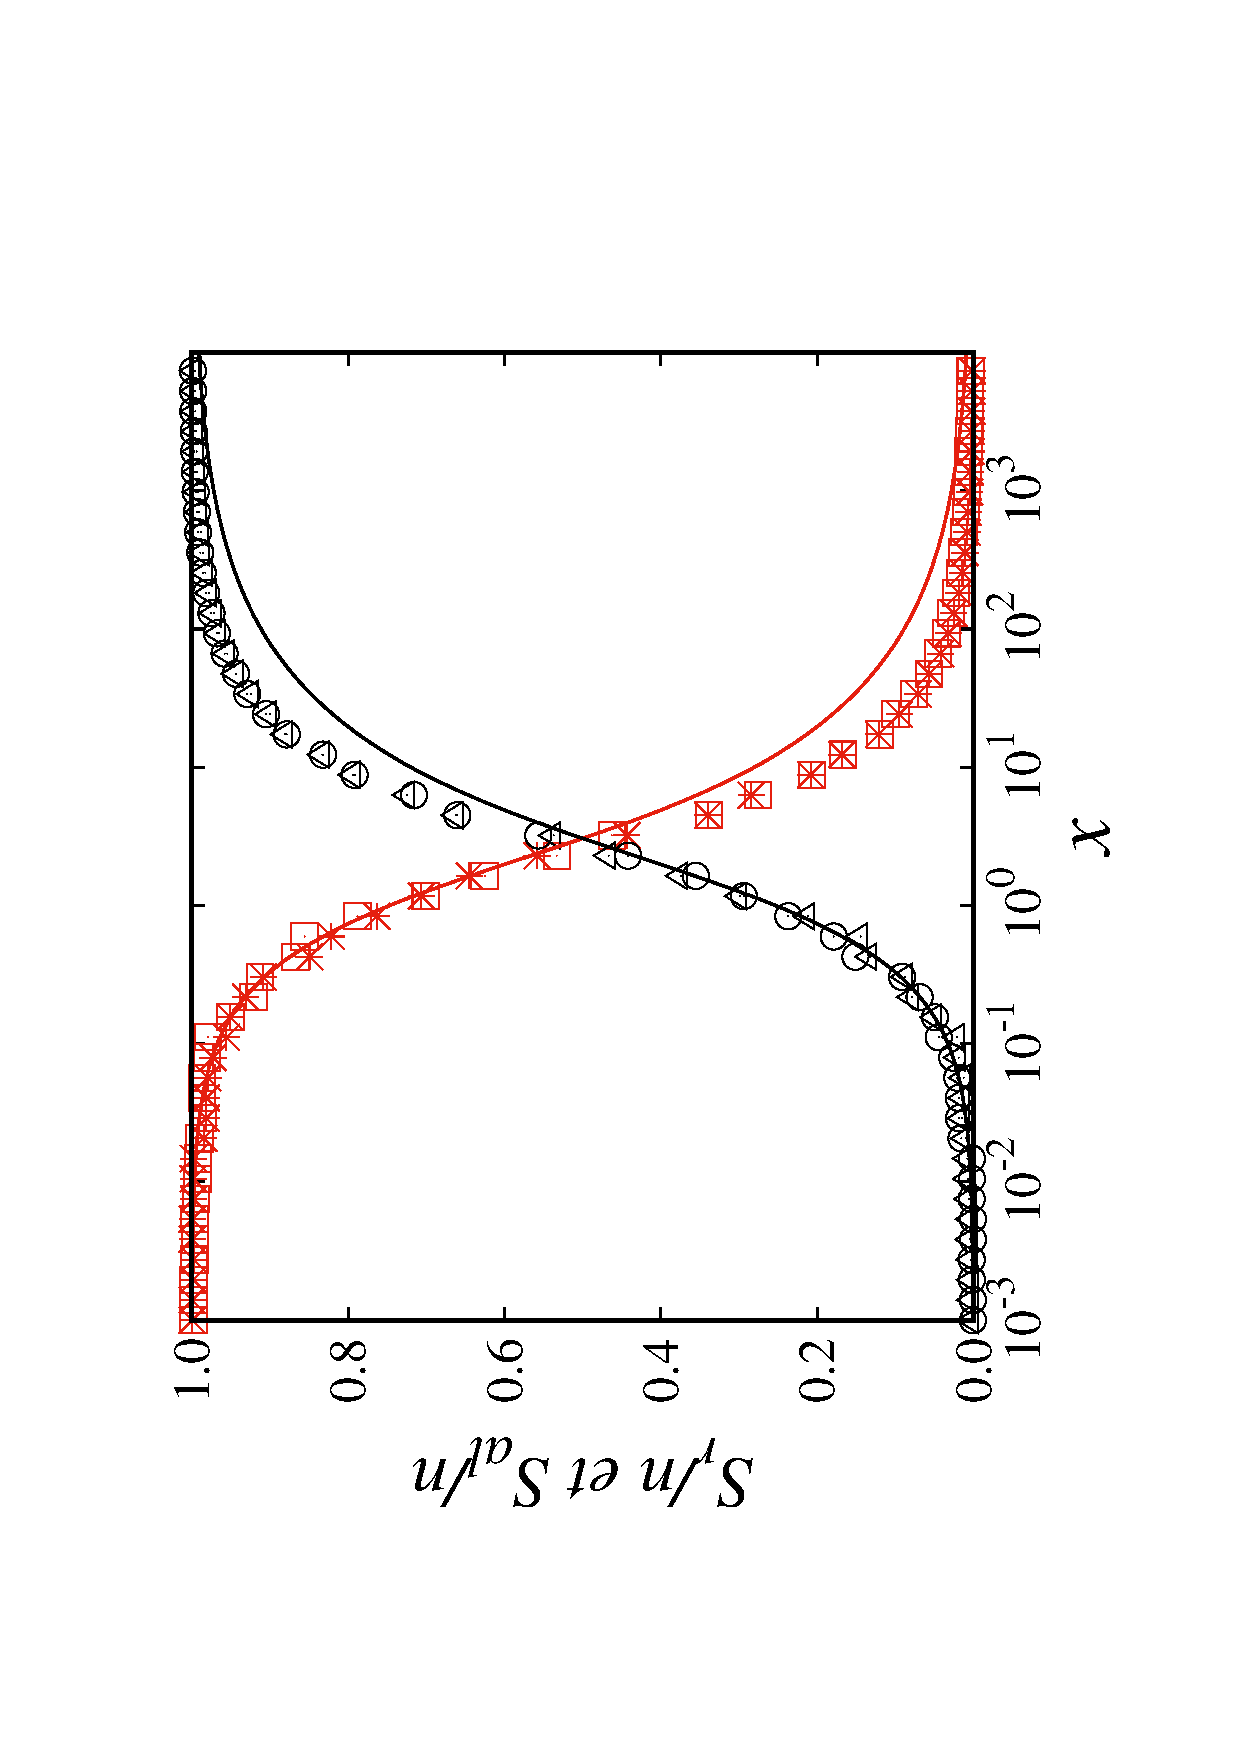
\includegraphics[scale=0.5,angle=-90]{./figures/fig-s}
	\caption{Fraction des nœuds aléatoires $\frac{S_{al}}{n}$ (noir) et des nœuds réguliers $\frac{S_{r}}{n}$ (rouge)  en fonction du nombre des raccourcis $x$. Les lignes représentent les deux fonctions $h(x)$  (noir) et $1-h(x)$ (rouge). Les symboles représentent les simulations numériques d'un réseau de taille $n=10^4$, avec $k=1$ (étoile et cercle) et $k=5$ (carré et triangle). Chaque simulation est moyennée sur $200$ réalisations. L'échelle est linéaire-log}
	\label{S}
\end{figure}
Les valeurs de $\hat{S}_{r}$ et $\hat{S}_{al}$ représentent en réalité le nombre des "\textsf{\textsf{amas}}" constitués de $k$ nœuds dans la transformation du GR,
alors pour trouver le nombre réel des nœuds dans le réseau il suffit de multiplier $\hat{S}_{r}$ et $\hat{S}_{al}$  par $k$,  d'où le nombre des nœuds réguliers est $S_r=n(1-h(kn\phi))$ et le nombre de nœuds aléatoires est $S_{al}=n h(kn\phi)$, où $h(x)$ est une fonction universelle qui représente la fraction des noeuds aléatoires.
%La fonction $h(x)$ peut être considérée comme un paramètre d'ordre. L'ordre représente la régularité du réseau. Sans raccourcis $h=1$,  l'ordre on peut conclure, selon son expression, qu'il \hat{n}y a pas une transition de phase dans ce modèle mais un phénomène de croisement qui commence depuis $x=0$. 
La Fig.~\ref{S} représente la variation des fractions des noeuds aléatoires et réguliers en fonction du nombre de raccourcis. Pour différentes valeurs du paramètre $k$, on a le même comportement de  $\frac{S_{r}}{n}$ et $\frac{S_{al}}{n}$, ce qui confirme l'universalité de ces deux grandeurs. Une observation importante est que pour $x\le1$ nos équations sont parfaitement en accord avec la simulation. Lorsque $x>1$ cet accord devient moins bon, ceci n'a rien de surprenant puisque les expressions de $S_{r}$ et $S_{al}$ ont été obtenus à partir de l'Eq.~\ref{ssr} en supposant que $\hat{\phi}$ (donc $x$) est petit.\\
Comme nous l'avons déjà mentionné, l'une des questions les plus intéressante dans le modèle de NW est l'existence ou non d'une transition de phase lors du passage du petit vers le grand monde. La quantité $\frac{S_{r}}{n}$ peut être considérée comme un éventuel paramètre d'ordre. L'ordre dans ce cas est la régularité du réseau, c'est-à-dire l'absence des raccourcis avec $\frac{S_{r}}{n}=1$. \`{A} partir d'un certain nombre de raccourcis $\frac{S_{r}}{n} \longrightarrow 0$, le réseau est desordonné. Il est pratiquement impossible de se prononcer sur l'existence de la transition de phase en étudiant le comportement de  $\frac{S_{r}}{n}$ (Fig.~\ref{S}). En général ce sont les fluctuations des grandeurs pertinentes qui peuvent donner l'information sur l'existence et la nature des transitions de phase. La Fig.~\ref{fluct} représente les fluctuations de $\frac{S_{al}}{n}$, soit  $\sigma=\frac{\sqrt{\textless{( \frac{S_{al}}{n})}^2\textgreater-\textless \frac{S_{al}}{n}\textgreater^2}}{\textless \frac{S_{al}}{n}\textgreater}$, en fonction du nombre de raccourcis  pour différentes valeurs de $n$. On remarque l'absence d'une divergence typique d'une transition de phase dans $\sigma$, qui présente un maximum au voisinage de $x=4.6$. Cette allure de $\sigma$ rappelle la forme de la chaleur spécifique en fonction de la température pour les systèmes paramagnétiques, et qui présente aussi un maximum appelé anomalie de Schottky.  

\begin{figure}[h!]
	\centering
	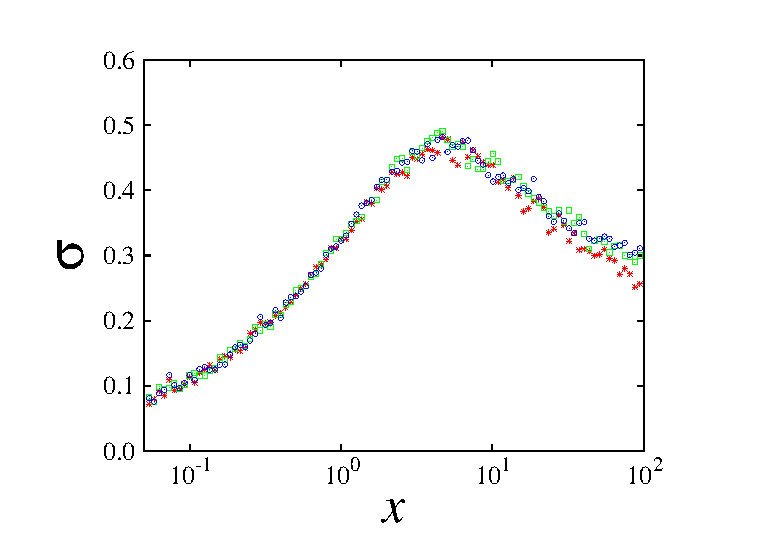
\includegraphics[scale=1,angle=0]{./figures/fluct}
	\caption{Fluctuation $\sigma$ en fonction de $x$ d'un réseau de $k=1$  pour différents valeurs de $n$, $n=10^3$ (étoile), $n=10^4$ (carré) et $n=10^5$ (cercle), le nombre de réalisations est $1000$. L'échelle est semi-logarithmique}
	\label{fluct}
\end{figure}
\subsection{Plus court chemin}
Le plus court chemin dans le réseau circulaire est donné par $\textless \hat{\ell} \textgreater=\sum_{\hat{\ell}=1}^{\frac{\hat{n}}{2}}(\hat{\ell}\cdot \hat{n}_{\hat{\ell}})\approx \int_1^{\frac{\hat n}{2}} \hat{\ell}\cdot \hat{n}_{\hat{\ell}} \cdot d\hat{\ell}$, où $\hat{n}_{\hat{\ell}}$ est le nombre de noeud a une distance $\hat{\ell}$. Pour faciliter les calculs on  introduit  $\textless \hat{\ell}_r \textgreater$ et $\textless\hat{\ell}_{al}\textgreater$ qui sont respectivement le plus court chemin des réseaux réguliers et aléatoires. Le réseau régulier est formé des noeuds dont la distance n'a pas été modifiée par l'ajout des raccourcis, et le réseau aléatoire est formé des noeuds dont la distance initiale a été changée après l'ajout des raccourcis. Le plus court chemin  du réseau global est $\textless \hat{\ell} \textgreater=\textless \hat{\ell}_r \textgreater+ \textless \hat{\ell}_{al} \textgreater$. 
Le plus court chemin du réseau régulier $\hat{\ell}_r$ s'écrit sous la forme 
\begin{equation}
\textless \hat{\ell}_r \textgreater=\frac{\hat{S}_r}{\hat{n}}\frac{\int_1^{\frac{\hat{n}}{2}}\hat{\ell}\cdot \hat{n}_{\hat{\ell}}^{r}d\hat{\ell}}{a_r},
\end{equation}
avec $a_r=\int_1^{\frac{\hat{n}}{2}}n_{\hat{\ell}}^{r}d\hat{\ell}=\hat{S}_r$
est la constante de normalisation, d'où $\textless \hat{\ell}_r \textgreater=\int_1^{\frac{\hat{n}}{2}}\hat{\ell}\cdot\frac{\hat{n}_{\hat{\ell}}^{r}}{\hat{n}}d\hat{\ell}$.\\
En utilisant les  Eq.~\eqref{pr} et Eq.~\eqref{cr} on obtient
\begin{eqnarray}
\textless \hat{\ell}_r \textgreater&=&\frac{1}{\hat{n}}\int^{\frac{\hat{n}}{2}}_1 2\hat{\ell}e^{-4\hat{\phi}\int_{j=1}^{\hat{\ell}-1}(j-1)(\hat{\phi}(\hat{n}-2j)+1)^{j-2}dj}d\hat{\ell},\nonumber
\end{eqnarray}
comme dans le cas de l'Eq.~\eqref{ssr} on prend $\hat{\phi}$ petit, ce qui donne 
\begin{eqnarray}\nonumber
\textless \hat{\ell}_r \textgreater &\approx&\frac{1}{\hat{n}}\int_1^{\frac{\hat{n}}{2}}2\hat{\ell}e^{-2\hat{\phi}\hat{\ell}^2}d\hat{\ell} \\\nonumber
&\approx&\frac{1}{\hat{n}}\frac{e^{-2\hat{\phi}}-e^{-\frac{\hat{\phi}\hat{n}^2}{2}}}{2\hat{\phi}}\\\nonumber
&\approx&\frac{1}{\hat{n}}\frac{1-e^{-\frac{\hat{\phi}\hat{n}^2}{2}}}{2\hat{\phi}} \quad \quad  \text{car:} \quad \hat{\phi}\ll1 \\
&\approx&\frac{\hat{n}}{4}\frac{1-e^{-\frac{\hat{\phi}\hat{n}^2}{2}}}{\frac{\hat{\phi}\hat{n}^2}{2}}.
\end{eqnarray}
Or $\frac{\hat{\phi}\hat{n}^2}{2}=nk\phi=x$ et $\hat{n}=\frac{n}{k}$, alors $\textless \hat{\ell}_r \textgreater$ peut s'écrire sous la forme universelle suivante
\begin{eqnarray}
\textless \hat{\ell}_r \textgreater&\approx&\frac{n}{k}\hat{f}_r(x) \quad \quad \textrm{avec} \quad \hat{f}_r(x)=\frac{1-e^{-x}}{4x}.
\label{lr}
\end{eqnarray}
Pour calculer $\textless \hat{\ell}_{al} \textgreater$, nous cherchons la position de la couche contenant le plus de noeud (voir Section.~\ref{pcc}), dans notre cas c'est le maximum de  $\hat{n}_{al}$. Explicitement, on résout l'équation $\frac{\partial \hat{n}_{al}(\hat{\ell})}{d\hat{\ell}}=0$. Des Eq.~\eqref{pr} et Eq.~\eqref{pal} on obtient :
\begin{eqnarray}
P_{al}(\hat{\ell})=u(\hat{\ell})e^{-\int_{j=1}^{\hat{\ell}-1}u(j)dj},
\label{Pal}
\end{eqnarray}
où 
\begin{eqnarray}
u(\hat{\ell})=4\hat{\phi}(\hat{\ell}-1)(\hat{\phi}(\hat{n}-2\hat{\ell})+1)^{\hat{\ell}-2}.
\label{ul}
\end{eqnarray}
Il est évident que $\textless \hat{\ell}_{al} \textgreater$ prédomine dans $\textless \hat{\ell} \textgreater$ si $S_{al}\gg S_r$, or la valeur du plus court chemin dans les réseaux aléatoires est de l'ordre de $\log(n)$ qui est très inférieure devant $\hat{n}$. On peut donc considérer que $\hat{n}-2\hat{\ell}\approx \hat{n}$, donc
$u(\hat{\ell})=4\hat{\phi}(\hat{\ell}-1)(\hat{\phi}\hat{n}+1)^{\hat{\ell}-2}$. Soit  $y=\hat{\phi}\hat{n}=2k^2\phi$, le paramètre qui représente le nombre moyen de raccourcis pour chaque \textsf{amas} après la transformation de GR, car $\hat{\phi}$ est la probabilité pour qu'un pair d'\textsf{\textsf{amas}} se connecte et $\hat{n}$ est le nombre d'\textsf{\textsf{amas}}.\\



 Des Eq.~\eqref{cal} et Eq.~\eqref{Pal} on obtient
\begin{eqnarray}
\hat{n}_{al}(\hat{\ell})=\hat{n}u(\hat{\ell})e^{-\int_{j=1}^{\hat{\ell}-1}u(j)dj},
\end{eqnarray}
donc 
\begin{eqnarray}
\frac{\partial \hat{n}_{al}(\hat{\ell})}{\partial \hat{\ell}}&=&\hat{n}\frac{\partial u(\hat{\ell})}{\partial \hat{\ell}}e^{-\int_{j=1}^{\hat{\ell}-1}u(j)dj}+\hat{n}u(\hat{\ell})\frac{\partial e^{-\int_{j=1}^{\hat{\ell}-1}u(j)dj}}{\partial \hat{\ell}}\\\nonumber
&=&\hat{n}\frac{\partial u(\hat{\ell})}{\partial \hat{\ell}}e^{-\int_{j=1}^{\hat{\ell}-1}u(j)dj}-\hat{n}u(\hat{\ell})^2e^{-\int_{j=1}^{\hat{\ell}-1}u(j)dj},\nonumber
\end{eqnarray}
alors le maximum de $\hat{n}_{al}$ est donnée par la solution de l'équation suivante
\begin{equation}
\frac{\partial u(\hat{\ell})}{\partial \hat{\ell}}-u(\hat{\ell})^2=0.
\label{28}
\end{equation}
D'après l'Eq.~\eqref{ul} on a $\frac{\partial u(\hat{\ell})}{\partial \hat{\ell}}=u(\hat{\ell})\big[\frac{1}{\hat{\ell}-1}+\ln(y+1)\big]$. Puisque $y=2k^2\phi$ ne dépend pas de la taille du réseau $\hat{n}$ alors que  $\hat{\ell}$ croît avec $\hat{n}$ on peut négliger $\frac{1}{\hat{\ell}-1}$ devant $\ln(y+1)$, on obtient $\frac{\partial u(\hat{\ell})}{\partial \hat{\ell}}=u(\hat{\ell})ln(y+1)$. L'Eq.~\eqref{28} devient
\begin{equation}
u(\hat{\ell})=\ln(y+1),
\label{29}
\end{equation}
En remplaçant $u(\hat{\ell})$ par son expression (Eq.~\eqref{ul}) on trouve la solution de l'Eq.~\eqref{29} qui  
donne la position $\hat{\ell}_{max}$ de $\hat{n}_{al}$ maximale:
\begin{equation}
\hat{\ell}_{max}=\frac{W\big(\frac{\ln(y+1)^2(y+1)}{4\hat{\phi}}\big)}{\ln(y+1)}+1,
\end{equation}
avec $W(x)$ est la fonction de Lambert.\\
Pour obtenir l'expression de $\textless \hat{\ell}_{al} \textgreater$ on multiplie $\hat{\ell}_{max}$  par la fraction des nœuds aléatoires: $\textless \hat{\ell}_{al} \textgreater=\hat{\ell}_{max}h(x)$, d'où 
\begin{equation}
\textless \hat{\ell}_{al} \textgreater=(\frac{W\big(\frac{\ln(y+1)^2(y+1)}{4\hat{\phi}}\big)}{\ln(y+1)}+1)h(x).
\label{lal}
\end{equation}
On peut écrire finalement l'expression du plus court chemin dans le modèle de NW en sommant les Eq.~\eqref{lr} et Eq.~\eqref{lal}: 
\begin{equation}
\textless \hat{\ell} \textgreater=\bigg(\frac{W\big(\frac{\ln(y+1)^2(y+1)}{4\hat{\phi}}\big)}{\ln(y+1)}+1\bigg)h(x)+\hat{n}\frac{1-e^{-x}}{4x}.
\label{l}
\end{equation}
\begin{figure}[h!]
	\centering
	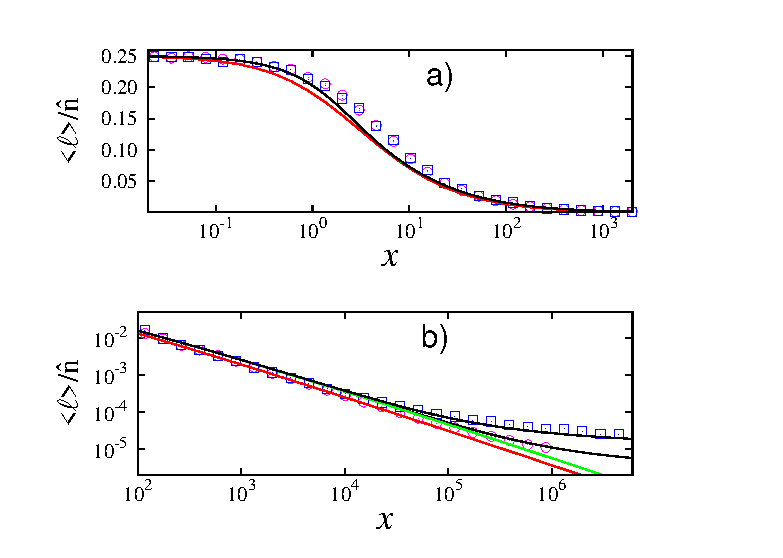
\includegraphics[scale=1.25,angle=0]{./figures/kpn}
	\caption{Comportement de  $\frac{\textless \hat{\ell} \textgreater}{\hat{n}}$ en fonction de $x$ pour un réseau de taille $n=10^6$. La formule de Newman et watts Eq.~\eqref{eq-ws} (ligne rouge), Eq.~\eqref{l2} (ligne verte), Eq.~\eqref{l} (ligne noire) et les simulations numériques pour $k=1$ (cercle) et $k=5$ (carré). L'échelle est semi-logarithmique dans \textbf{a)} et log-log dans \textbf{b)}. Chaque simulation est moyennée sur $100$ réalisations.}
	\label{chemin}
\end{figure}
Pour trouver une expression universelle de $\textless \hat{\ell} \textgreater$ en fonction du nombre de raccourcis $x$, il faut prendre $y\ll 1$ dans l'équation Eq.~\eqref{l},  soit: \footnote{Cette condition n'est pas toujours vraie, ceci sera discuté par la suite.}.
\begin{eqnarray}
\textless \hat{\ell} \textgreater=\hat{n}\hat{f}(x), 
\label{l2}
\end{eqnarray}
avec $\hat{f}(x)=\big(\frac{2W(\frac{x}{2})h(x)+1-e^{-x}}{4x}\big)$ est la fonction universelle.\\
De la Fig.~\ref{chemin}, on voit que l'Eq.~\eqref{l} est en très bon accord avec les simulations en dehors de l'intervalle $]1,10]$. La Fig.~\ref{chemin}(b) montre que l'Eq.~\eqref{l} est plus précise que l'Eq.~\eqref{eq-ws} de Newman et al. notamment pour les grandes valeurs de $x$. L'intervalle $]1,10]$ où notre théorie est en désaccord avec la simulation correspond dans la Fig.~\ref{fluct} au maximum de fluctuations du paramètre $\frac{S_{al}}{n}$, donc c'est l'intervalle où notre approximation qui est de champ moyen est moins précise.

\section{Émergence de la propriété petit-monde dans le modèle de NW}
\subsection{Validité de la fonction universelle de NW}
L'expression universelle $\frac{\textless {\ell} \textgreater}{\hat{n}}={f}(x)$ est obtenue pour $y\ll 1$, ceci va être confirmé dans ce qui suit par les simulations. Pour cela on définit $\Delta$ tel que:
\begin{equation}
\Delta= \frac{\frac{\textless {\ell} \textgreater}{\hat{n}}}{f(x)},
\end{equation}
de sorte que si la fonction $f(x)=\frac{\textless {\ell} \textgreater}{\hat{n}}$ est universelle, alors  $\Delta$ doit être égale $1$.
\begin{figure}[h!]
	\centering
	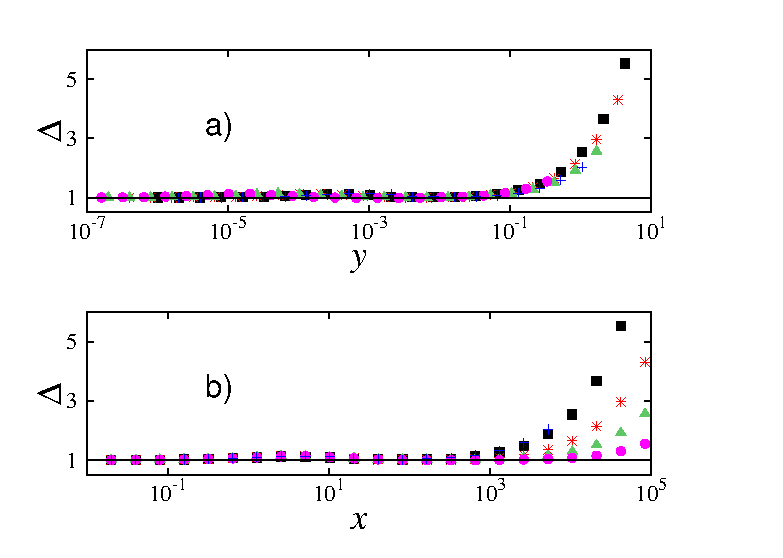
\includegraphics[scale=0.95,angle=0]{./figures/def}
	\caption{Variations de $\Delta$ en fonction de $y$ (a)  et $x$ (b) pour différentes valeurs de $n$ et $k$. $k=1$ et $n=10^{5}$ (triangle),	$k=2$ et $n=10^{4}$ (plus),  $k=2$ et $n=10^{6}$ (cercle), $k=2$ et $n=10^{5}$ (étoile), $k=5$ et $n=10^{6}$ (carré). Le nombre de réalisations pour chaque simulation est $1000$. L'échelle est semi-logarithmique}
	\label{def}
\end{figure}\\
Dans la Fig.~\ref{def} on représente $\Delta$ en fonction de $y$ et $x$, $\textless \ell \textgreater$ est obtenu par simulation du modèle de NW, et $f(x)$ est l'Eq.~\eqref{eq-ws}. On observe que $\Delta$ est effectivement égale $1$ pour $y\ll1$. Pour les valeurs supérieures de $y$, $\Delta$ est nettement supérieur à $1$, par conséquent $f(x)$ n'est plus valable.  \footnote{Newman a déjà soulevé le problème avec $f(x)$ lorsque $\phi=1$ \cite{Newman-al2000} .}. La Fig.~\ref{def}(b) montre aussi que la fonction $f(x)$ n'est pas universelle à partir d'une certaine valeur de $x$ qui dépend des paramètres du réseau. Les Fig.~\ref{def}(b) et Fig.~\ref{chemin} suggèrent que le rapport $\frac{\textless {\ell} \textgreater}{\hat{n}}$ ne peut être écrit sous forme d'une fonction universelle du paramètre $x=nk\phi$. En d'autres termes, et en suivant l'argumentation de Newman \cite{Newman-al2000}, il faut chercher à exprimer le plus court chemin en fonction d'autres paramètres.
\section{Une nouvelle fonction universelle }
L'universalité de $\Delta$ en fonction du paramaètre $y$ (Fig.~\ref{def}(a)) et le changement de son comportement à partir d'une certaine valeur de $y$ nous a poussé à representer $\frac{\ln(n)}{\textless {\ell} \textgreater}$ en fonction de ce paramètre (Fig.~\ref{fu}). L'idée est de voir si ce changement est lié au passage du réseau grand monde lorsque $\textless {\ell} \textgreater \propto n $ au petit monde lorsque $\textless {\ell} \textgreater \propto \ln(n)$. On observe dans la Fig.~\ref{fu} que lorsque $y\ll1$ on a $\frac{\ln(n)}{\textless {\ell} \textgreater}\longrightarrow 0$, ce qui correspond au comportement grand monde du réseau car dans ce cas $\textless {\ell} \textgreater \propto n$, par contre lorsque $y$ n'est plus très inférieur à $1$, $\textless {\ell} \textgreater \propto \ln(n)$, ce qui correspond au comportement petit monde Un résultat très important ici est que lorsque le réseau est petit monde c'est $\frac{\textless {\ell} \textgreater}{\log(n)}$ qui est universelle et non pas $\frac{\textless {\ell} \textgreater}{n}$ comme dans \cite{Newman-Watts1999-2}. En outre $\frac{\textless {\ell} \textgreater}{\log(n)}$ doit être exprimée en fonction de $y$ et non pas en fonction de $x$.
%Comme nous l'avons déjà signalé, la non validité de la fonction universelle de NW peut signifier que le réseau commence à posséder la propriété petit monde,
%autrement dit le plus court chemin devient de l'ordre de $\ln(n)$, pour confirmer cette %hypothèse on va faire des simulations numériques et puis on  va les comparer avec notre expression théorique.\\
%En effet, Si on trace l'expression
% $\frac{\ln(n)}{\ell}$ en fonction de $y$ on remarque une émergence universelle de celui-ci . On en déduit alors qu'une nouvelle fonction universelle sous la forme $g(y)=\frac{\ln(n)}{\hat{\ell}}$  est apparaît.\\
%Ce changement de comportement reflète le passage du grand monde lorsque $y$ est petit \footnote{Lorsque $y$ est petit, le nombre de raccourcis dans le réseau est forcément petit.} au petit monde pour $y$ suffisamment élevé. De plus à partir des Fig.~\ref{def}(a) et Fig.~\ref{def}(b) on remarque que ce passage de grand monde au petit monde se fait en fonction de $y$ et pas de $x$ (la Fig.~\ref{fu} montre bien cette hypothèse). En outre, la Fig.~\ref{chemin}(b)
%montre également que lorsque le réseau est petit monde, la fonction $f(x)$ n'est pas universelle. 
Pour trouver l'expression analytique de la nouvelle fonction universelle $g(y)$ telle que $g(y)=\frac{\textless {\ell} \textgreater}{\ln(n)}$ on prend $n$ grand dans l'Eq.~\eqref{l}. Dans ce cas $W\big(\frac{\ln(y+1)^2(y+1)}{4\hat{\phi}}\big)\approx \ln \big(\frac{\ln(y+1)^2(y+1)}{4\hat{\phi}}\big)$,  $h(x)=1-\sqrt{\frac{\pi}{4x}}erf(\sqrt{x}) \longrightarrow 1$, et $\frac{y+1}{4\hat{\phi}}=n\frac{2k^2\phi+1}{8k^3\phi}$. D'autre part, le réseau est petit monde si $y$ n'est pas très inférieur à $1$ (Fig.~\ref{fu}). L'eq.~\eqref{l} devient:
\begin{eqnarray}
\textless {\hat\ell} \textgreater&=&\frac {\ln \ln(y+1)^2+\ln \frac{y+1}{4\hat{\phi}}}{\ln(y+1)}+1+\frac{1-e^{-x}}{2y} \nonumber\\
&\approx& \frac{\ln n}{\ln(y+1)}
\label{lc}
\end{eqnarray}
\begin{figure}[h!]
	\centering
	%	\begin{tikzpicture}
	\begin{tikzpicture}
	%\draw (4,-20) ellipse (2cm and 1cm) ;
	%\end{tikzpicture}
	%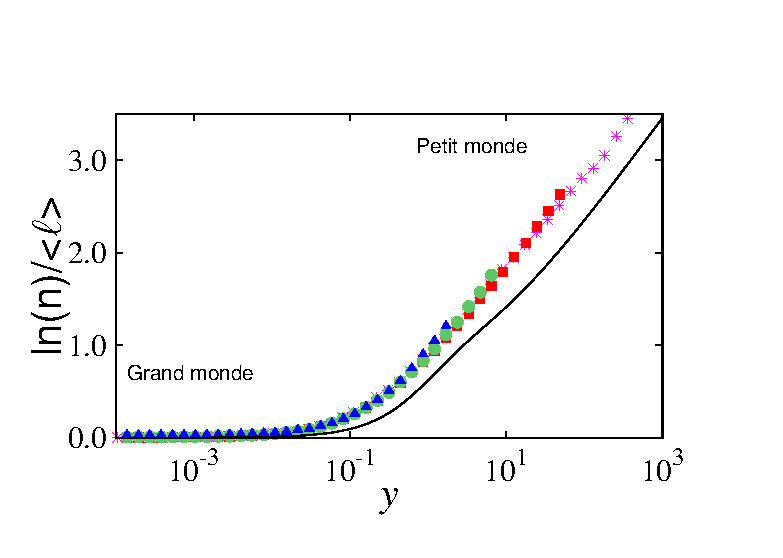
\includegraphics[scale=1,angle=0]{./figures/kp};
	\pgftext{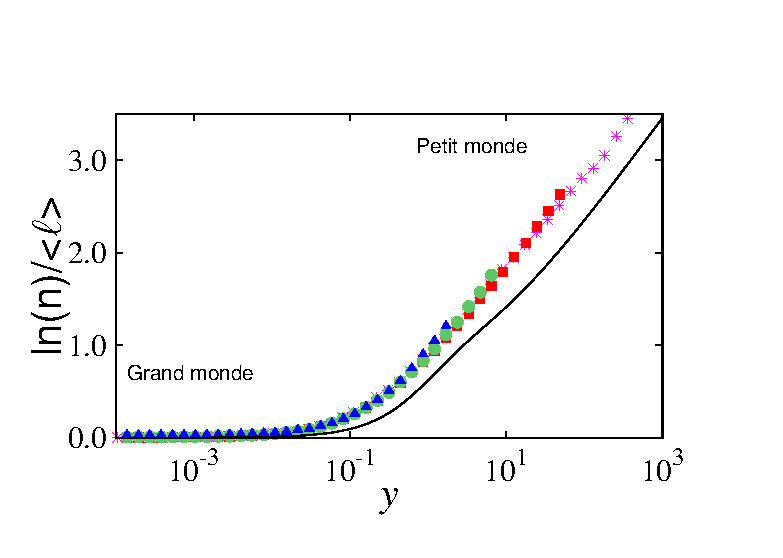
\includegraphics[scale=1]{./figures/kp}} at (0pt,0pt);
	\draw[line width=2pt] (-3.5,-2.7) ellipse (1cm and 0.5cm) ;
	\draw[line width=2pt,rotate=45] (2.2,-1.2) ellipse (2.2cm and 0.95cm) ;
	\end{tikzpicture}
	\caption{$\frac{\ln(n)}{\textless {\ell} \textgreater}$ en fonction de $y$. La ligne continue est l'Eq.~\eqref{kp2}, les symboles représentent les simulations numériques pour différents valeurs de $n$ et $k$: $n=10^{-6}$ et $k=20$ (étoile), $n=10^{-5}$ et $k=5$ (carré), $n=10^{-4}$ et $k=2$ (cercle),$n=10^{-3}$ et $k=1$ (triangle), nombre de réalisations pour chaque simulations est $100$. L'échelle est semi-logarithmique.}
	\label{fu}
\end{figure}
$\textless {\hat\ell} \textgreater$ est le plus court chemin entre les \textsf{amas} du réseau issus de la transformation GR, pour obtenir le plus court chemin $\textless \ell \textgreater$ entre deux noeuds dans le réseau de NW, on cherche la relation entre les deux quantités en utilisant l'approximation suivante:
Entre deux \textsf{\textsf{amas}} quelconques dans le réseau il peut y avoir des liens ordinaires et/ou des raccourcis. Dans le cas où il y a deux raccourcis liés au m\^{e}me \textsf{\textsf{amas}} intermédiaire (Fig.~\ref{recul}), la probabilité qu'ils soient liés au m\^{e}me nœud dans cet \textsf{\textsf{amas}} est $\frac{1}{k}$ (Fig.~\ref{recul}(b)), et la probabilité que les deux raccourcis ne soient pas liés au m\^{e}me nœud (Fig.~\ref{recul}(a)), donc faisant intervenir un autre lien, est  $1-\frac{1}{k}$, autrement dit chaque fois qu'on a deux raccourcis pointant vers le même \textsf{amas} il y a une probabilité de $1-\frac{1}{k}$ que le plus court chemin augmente de $1$.\\
D'autre part, le nombre de liens réguliers entre les \textsf{\textsf{amas}} est toujours
$\hat{n}$, et le nombre de raccourcis entre les \textsf{\textsf{amas}} est $\frac{\hat{\phi}\hat{n}(\hat{n}-1)}{2}\approx\frac{\hat{\phi}\hat{n}^2}{2}$,
$\hat{\phi}$ est la probabilité qu'une paire d'\textsf{\textsf{amas}} se connecte par un raccourci et $\frac{\hat{n}(\hat{n}-1)}{2}$ est le nombre de paires possibles. Alors la fraction de raccourcis par rapport au nombre total de liens est $\frac{\hat{\phi}\hat{n}}{2+\hat{\phi}\hat{n}}=\frac{y}{2+y}$, d'où la probabilité d'obtenir deux raccourcis liés au m\^{e}me \textsf{\textsf{amas}} entre deux nœuds quelconques du réseau est $(\frac{y}{2+y})^2$. Par conséquent la probabilité pour que la valeur du plus court chemin entre deux \textsf{amas} soit doublée est $(\frac{y}{2+y})^2(1-\frac{1}{k})$. La probabilité que le plus court chemin reste inchangé est $(1-(\frac{y}{2+y})^2)+\frac{1}{k}(\frac{y}{2+y})^2$, le première terme représente la probabilité que deux raccourcis ne soient pas liés au m\^{e}me \textsf{\textsf{amas}} et le deuxième représente la probabilité 
que deux raccourcis soient liés au m\^{e}me \textsf{\textsf{amas}} et également au m\^{e}me nœud, ceci se traduit par: 
\begin{eqnarray}
\textless {\ell} \textgreater=\textless {\hat \ell} \textgreater \Bigg[\frac{1}{k}(\frac{y}{2+y})^2+(1-(\frac{y}{2+y})^2)+2(1-\frac{1}{k})(\frac{y}{2+y})^2\Bigg],
\end{eqnarray}
en remplaçant dans l'Eq.~\eqref{lc}, on déduit:
\begin{eqnarray}
\frac{\textless {\ell} \textgreater}{\ln(n)}=\frac{\frac{1}{k}(\frac{y}{2+y})^2+(1-(\frac{y}{2+y})^2)+2(1-\frac{1}{k})(\frac{y}{2+y})^2}{\ln(y+1)},
\end{eqnarray}
en prenant $\frac{1}{k}\ll1$ on obtient:
\begin{eqnarray}
\frac{\textless {\ell} \textgreater}{\ln(n)}=\frac{\big(1+(\frac{y}{2+y})^2\big)}{\ln(y+1)}=g(y)
\label{kp2}
\end{eqnarray}

\begin{figure}[h!]
	\centering 
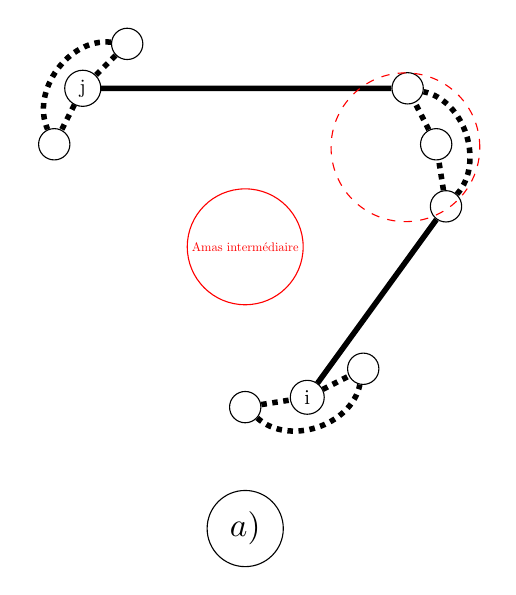
\begin{tikzpicture}[scale=0.3]
\draw (0,-12) node[scale=2,below]{$a)$} ;
\draw (0,0.75) node[scale=0.75,below,red]{Amas intermédiaire} ;
\tikzstyle{every node}=[scale=0.6,draw,shape=circle];
\node[scale=2] (5) at (0:8.5) {};
\node[scale=2] (6) at ( 18:8.5) {};
\node[scale=2] (7) at (2*18:8.5) {};
\node[scale=2] (12) at (7*18:8.5) {};
\node[scale=1.2] (13) at (8*18:8.5) {j};
\node[scale=2] (14) at (9*18:8.5) {};
\node[scale=2] (r) at (15*18:8.5) {};
\node[scale=1.25] (1) at (16*18:8.5) {i};
\node[scale=2] (2) at (17*18:8.5) {};
\draw[line width=2pt,dotted](r)--(1)
(1) -- (2)
(5) -- (6)
(6) -- (7)
(12) -- (13)
(13) -- (14);
\draw[line width=2pt](7) -- (13)
(1) -- (5);
\draw[line width=2pt,dotted] (r) to [bend right=60] (2) 
(12)to [bend right=60](14)
(5)to [bend right=60](7);
\filldraw[black] (3.5,2.5) node[scale=9.5,anchor=west,red,dashed] {};
\end{tikzpicture}
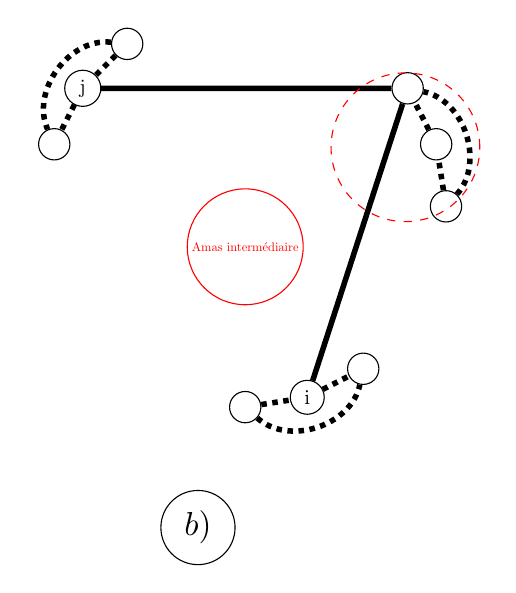
\begin{tikzpicture}[scale=0.3]
\draw (-2,-12) node[scale=2,below]{$b)$} ;
\draw (0,0.75) node[scale=0.75,below,red]{Amas intermédiaire} ;
\tikzstyle{every node}=[scale=0.6,draw,shape=circle];
\node[scale=2] (5) at (0:8.5) {};
\node[scale=2] (6) at ( 18:8.5) {};
\node[scale=2] (7) at (2*18:8.5) {};
\node[scale=2] (12) at (7*18:8.5) {};
\node[scale=1.2] (13) at (8*18:8.5) {j};
\node[scale=2] (14) at (9*18:8.5) {};
\node[scale=2] (r) at (15*18:8.5) {};
\node[scale=1.25] (1) at (16*18:8.5) {i};
\node[scale=2] (2) at (17*18:8.5) {};
\draw[line width=2pt,dotted](r)--(1)
(1) -- (2)
(5) -- (6)
(6) -- (7)
(12) -- (13)
(13) -- (14);
\draw[line width=2pt](1) -- (7)
(7) -- (13);
\draw[line width=2pt,dotted] (r) to [bend right=60] (2) 
(12)to [bend right=60](14)
(5)to [bend right=60](7);
\filldraw[black] (3.5,2.5) node[scale=9.5,anchor=west,red,dashed] {};
\end{tikzpicture}
\caption{Distance entre deux \textsf{amas} ayant un amas commun (intermédiaire) dans le réseau de NW, avec deux raccourcis (ligne continue) entres eux et  $k=3$. Les lignes en pointillés représentent les liens réguliers. Dans a) la distance entre le noeud $i$ et $j$ est $3$ car les deux raccourcis ne sont pas liés au même noeud de l'\textsf{amas} intermédiaire, dans b) la distance entre le noeud $i$ et $j$ est $2$ car les deux raccourcis  sont liés au même noued de l'\textsf{amas} intermédiaire.}
\label{recul}
\end{figure}
Cette fonction montre un certain écart par rapport aux résultats numériques, car dans la déduction de $\textless {\ell} \textgreater$ en fonction de $\textless {\hat \ell} \textgreater$  nous avons seulement pris en compte le cas de deux raccourcis liés au même \textsf{amas}, il s'agit donc d'une  approximation de type champs moyen. Cependant 
l'expression de $g(y)$  se compare qualitativement bien avec les simulations (Fig.~\ref{fu}).\\
Il convient de signaler que la fonction universelle $h$ est en fonction de $x$ et pas de $y$, car nous avons ignoré dans le calcul de $h(x)$ le cas où $\hat{\phi}$ est grand (donc $x$ est grand),  alors cette expression n'est valable que pour un petit nombre de raccourcis. 

\section{Conclusion}
Nous avons étudiant le modèle de NW d'une manière extensive, et nous avons introduit une nouvelle façon d'aborder ce système. En effet, afin d'obtenir plus d'informations sur les différents aspects du réseau, nous avons séparé la contribution des noeuds ``réguliers'' et ``aléatoires''. 
En utilisant la transformation de GR, nous avons pu calculer la fraction des noeuds ``réguliers''  ($S_r$) et ``aléatoires'' ($S_{al}$). En calculant les fluctuations de $\frac {S_r}{n}$ que nous avons considéré comme paramètre d'ordre, nous avons conclu qu'il n'y pas de transitions de phase de grand monde vers petit monde. \`{A} partir  de $S_r$ et $S_{al}$ nous avons déduit le plus court chemin $\textless {\ell} \textgreater$. Notre expression pour $\textless {\ell} \textgreater$ est plus précise que celle donnée par Newman et al. \cite{Newman-al2000}. En outre, cette expression nous amène à conclure que la fonction universelle de Newman et al. \cite{Newman-Watts1999-2} n'est valable que lorsque le réseau est grand monde, ce qui se traduit dans nos équations par $y=2k^2\phi \ll 1$. Lorsque le réseau est petit monde, nous avons proposé une nouvelle fonction universelle quit s'écrit en fonction de $y$.  En général, nous avons déduit que dans le modèle de NW, lorsque le réseau est grand le monde, la fonction universelle $(f(x))$ doit s'écrire en fonction de $x$ et le plus court chemin en fonction de $n$ et $x$, alors que lorsque le réseau est petit monde, la fonction universelle $(g(y))$ doit être fonction de $y$ et le plus court chemin en fonction de $y$ et $\ln(n)$.

